\documentclass[conference]{IEEEtran}

\usepackage{silence}
\WarningsOff[latexfont]

\newcommand{\subparagraph}{}

\usepackage{amsmath}
\usepackage[american]{babel}
\usepackage{booktabs}
\usepackage{multirow}
\usepackage[T1]{fontenc}
\usepackage[utf8]{inputenc}
\usepackage[binary-units,per-mode=symbol]{siunitx}
\usepackage[caption=false,font=footnotesize]{subfig}
\usepackage{xfrac}
\usepackage{xspace}
\usepackage{titlesec}
\usepackage{graphicx}
\usepackage{hyperref}
\usepackage[noabbrev,capitalise]{cleveref}

\setcounter{secnumdepth}{4}

\titleformat{\paragraph}
{\normalfont\normalsize\bfseries}{\theparagraph}{1em}{}
\titlespacing*{\paragraph}
{0pt}{3.25ex plus 1ex minus .2ex}{1.5ex plus .2ex}

\begin{document}

\title{Simplified wireless network simulation and analysis}

\author{
    \IEEEauthorblockN{Alessandro Pezzé, 182501}
    \texttt{alessandro.pezze@studenti.unitn.it}
}

\maketitle

\begin{abstract}
A simulator of a simple wireless network is derived from known given parameters, enough data is then gathered in order to perform an in-depth analysis of its behavior. Moreover, the sketch of a mathematical model of the wireless system is provided, along with its solution and a comparison with the coded simulator.
\end{abstract}

\section{Introduction}\label{sec:introduction}
A simple 10 nodes wireless network is simulated given \href{http://www.sharelatex.com}{a set of constraints} which can be summed up as follows:
\begin{itemize}
\item Each node resides in a unit square area and can broadcast to any other node within a range of 0.25 units
\item Each node generates a packet to be transmitted as soon as it can, with inter-arrival time being defined by an Exponential distribution. In order to study how the net performs in different conditions (high traffic, low traffic) the “rate” of the distribution is free.
\item Each packet has a size that follows a Binomial distribution \(B(p=0.806, n=1124)\) that cannot exceed a hard size limit of \([32, 1156]\).
\item The network rules are similar to the trivial continuous Pure ALOHA ones, and can be found in the Assignment paper.
\end{itemize}

\begin{figure}[h]
    \centering
    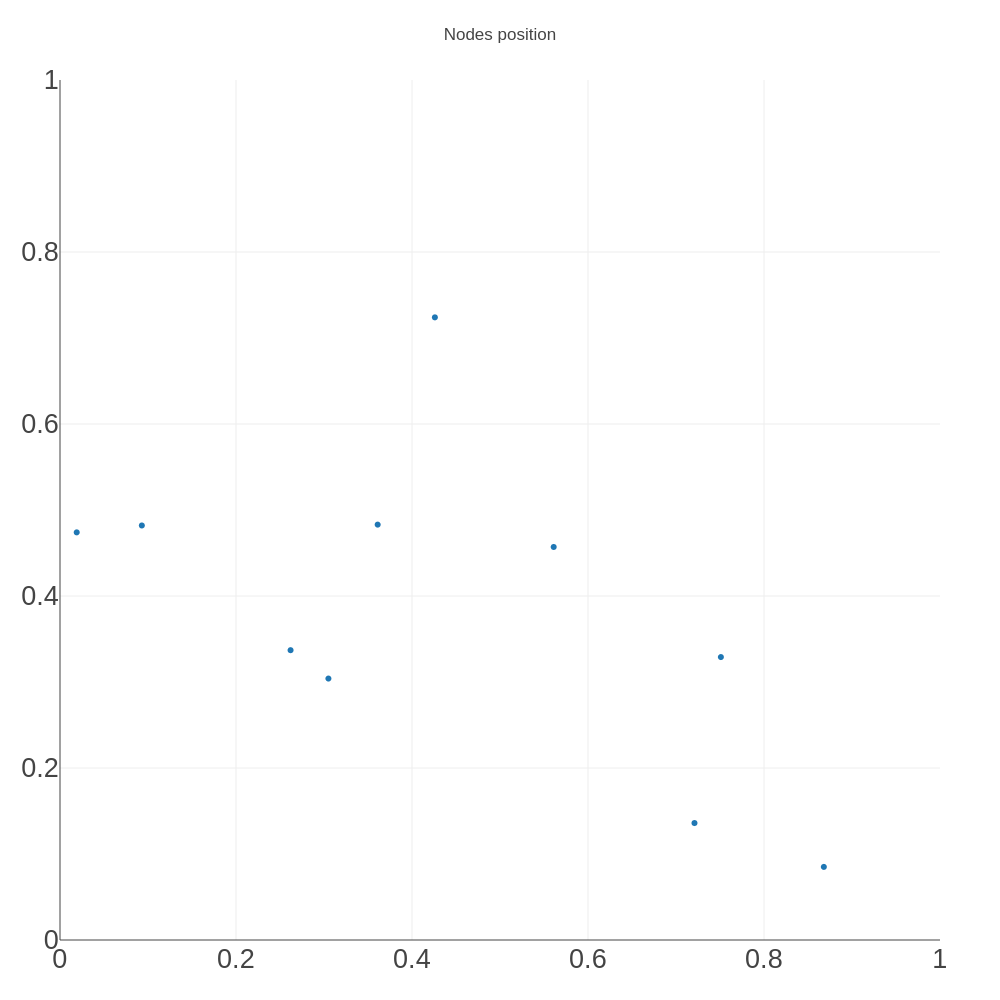
\includegraphics[width=\columnwidth]{graphs/NodesPositions}
    \caption{Node positions}
    \label{fig:nodespositions}
\end{figure}

\section{Simulation}\label{sec:simulation}

\subsection{Design}\label{sec:design}
A simple network simulator has been designed, with three actors taking the main roles: \(Packets\) sent across the channels; these \(Packets\) are generated by \(Nodes\); \(Nodes\) are controlled and orchestrated by a single \(Scheduler\). The role of the \(Scheduler\) is to manage the \(Events\) of the system using a heap queue, popping them as their turn to be executed comes. These \(Events\) are basically requests of \(Nodes\) to send \(Packets\). Each time a \(Node\) wants to send a \(Packet\) it has to file an \(Event\) to the \(Scheduler\), which will add the event to the queue in the correct order. When an \(Event\) is fired by the \(Scheduler\), the packet is extracted from the \(Event\) and the \(Node\) that generated it sends it over the network, eventually returning the control to the \(Scheduler\). If the \(Node\) was already sending another \(Packet\), the to-be-sent \(Packet\) is both pushed back in the \(Scheduler\) heap queue, and marked as 'queued' and pushed to the \(Node\)’s queue (which can contain up to 40 \(Packets\)). If no room is available in the \(Node\) queue, the \(Packet\) is discarded. If the \(Packet\) is sent to a \(Node\) that was already in a sending or receiving state, the \(Packet\) is considered 'collided'. After the \(Packet\) is sent, collided, or lost the \(Node\) in charge schedules for himself another \(Event\), based on the two distribution mentioned in the Introduction. This handling \(Events\) loop is then repeated for either a fixed interval of time, or for a fixed amount of steps. Figure 2 shows the entire flow of the simulator.

\begin{figure*}[t]
    \centering
    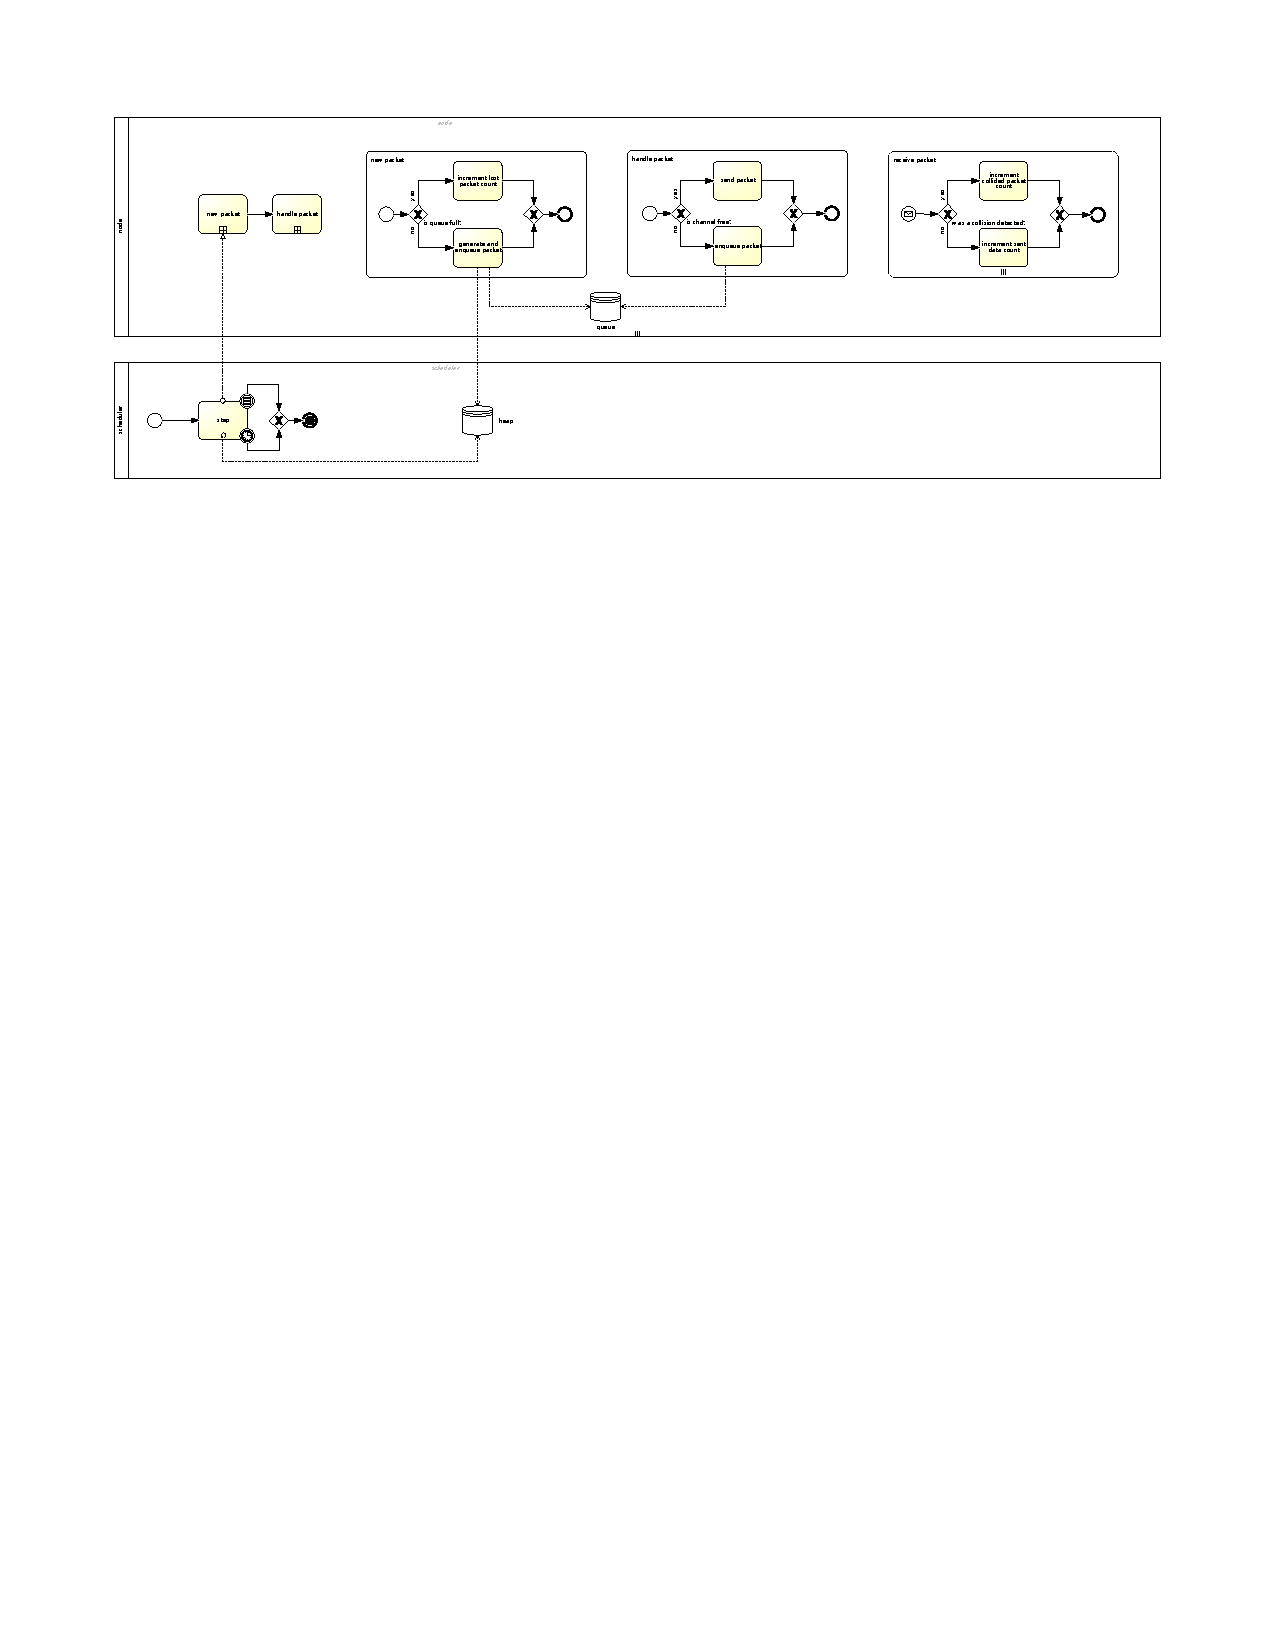
\includegraphics[width=\textwidth]{graphs/FlowChart}
    \caption{Simulator flow chart}
    \label{fig:flowchart}
\end{figure*}

\begin{table}
    \centering
    \caption{Main Python modules}
    \label{tab:mainpythonmodules}
    \begin{tabular}{l|l}
        \toprule
        module & description \\
        \midrule
        \(arguments.py\) & defines command line arguments \\
        \(iris.py\) & start a single simulation \\
        \(log.py\) & defines logging functions \\
        \(node.py\) & defines the node entity \\
        \(packet.py\) & defines the packet entity \\
        \(scheduler.py\) & defines the scheduler entity \\
        \(settings.py\) & contains general settings \\
        \bottomrule
    \end{tabular}
\end{table}

\subsection{Implementation}\label{sec:implementation}
To implement the simulator Python 3 was used, in order to take advantage of its OOP capabilities. The code was thus split between the actors of the simulator by defining the Scheduler, Node, and Packet classes. Among them, other helper classes have been defined in order to read the initially given settings, to read the command line arguments, to efficiently log the simulator state, and to start the simulator. A brief description of those classes can be found in \cref{tab:mainpythonmodules}. The source code for these classes is attached and can be easily accessed: it will thus not be explained in detail. It is particularly important to denote how the two distributions, packet size and inter-arrival time, were designed in Python: the third-party library “Numpy” was used, since it provided the methods to generate samples from both Binomial and Exponential distributions. The samples from the Binomial distributions were truncated in order to not exceed the maximum and minimum packet size \([32, 1156]\); to generate Exponential samples Numpy required the use of a Scale parameter \(\beta\) instead of the common Rate \(\lambda\) parameter, with \(\beta=1/\lambda\). In order to run the simulations enough times to gather all the necessary data, a Python script was coded to start sequential simulations with different parameters, like the parameter which rules the inter-arrival time distribution, or the seed which governs the random aspects of the simulation (i.e. the distributions). The simulation is ran with 100 different seeds for each of the scale parameters found in \cref{tab:scalevalues}. A Makefile is provided in order to run the entire simulation (\texttt{make run}) and to install a Python virtual environment with all the necessary dependencies (numpy among the others).

\begin{table}
    \centering
    \caption{\(\beta\) values}
    \label{tab:scalevalues}
    \begin{tabular}{cc|c}
        \toprule
        from & to & increment \\
        \midrule
        \num{0.00095} & \num{0.003} & \num{0.00005} \\
        \num{0.003} & \num{0.005} & \num{0.0004} \\
        \num{0.005} & \num{0.01} & \num{0.001} \\
        \num{0.01} & \num{0.02} & \num{0.004} \\
        \num{0.02} & \num{0.1} & \num{0.008} \\
        \bottomrule
    \end{tabular}
    
    The scale parameter is used in the simulator instead of the rate \(\lambda=1/\beta\), because the utilized mathematical module \href{https://docs.scipy.org/doc/numpy-1.13.0/reference/generated/numpy.random.exponential.html}{uses the scale parameter}.
\end{table}

\subsection{Execution}\label{sec:execution}
In order to execute the simulation a Linux machine with an distribution of Python 3.x installed is required. If such environment is not present, a \texttt{docker-compose.yml} file is provided to instantiate a proper Python 3 container. Moreover, provided the simulation is ran locally, the local installation of Python will not be polluted with the project dependencies, thanks to the creation of a Python virtual environment. In order to download all the dependencies the command \texttt{make} has to be ran in a first time. Then with the command \texttt{make run} a set of sequential simulations is started with different seeds and scale parameters.

\section{Evaluation}\label{sec:evaluation}

\subsection{Aggregation}\label{sec:aggragation}
The Python simulator described above stores its results in two \(CSV\) files, one for the single nodes and one for the total system seen as a single entity. The \(CSV\) files store the data as in \cref{tab:csvformat}, with the \(CSV\) file for the entire system lacking the node identifier. In order to analyze the data an R script was used: the data is loaded into an R data frame, and aggregated using the scale of the Exponential distribution as a point of aggregation, since it is the only free parameter of the system; a mean is then calculated over the aggregated elements . The rate parameter was derived from the scale parameter using \cref{eq:scaletorate} to better reflect the provided settings file. 

\begin{equation}
    \lambda=1/\beta\label{eq:scaletorate}
\end{equation}

\begin{table}
    \centering
    \caption{\(CSV\) format}
    \label{tab:csvformat}
    \begin{tabular}{l|l}
        \toprule
        value & description \\
        \midrule
        \(node\) & the node to which the data applies \\
        \(scale\) & value of the scale parameter \\
        \(throughput\) & the successful throughput of the system or the node \\
        \(load\) & the offered load of the system or the node \\
        \(collision\) & percentage of collided packets \\
        \(lost\) & percentage of packets lost due to full queues \\
        \bottomrule
    \end{tabular}
\end{table}

\begin{figure}[t]
    \centering
    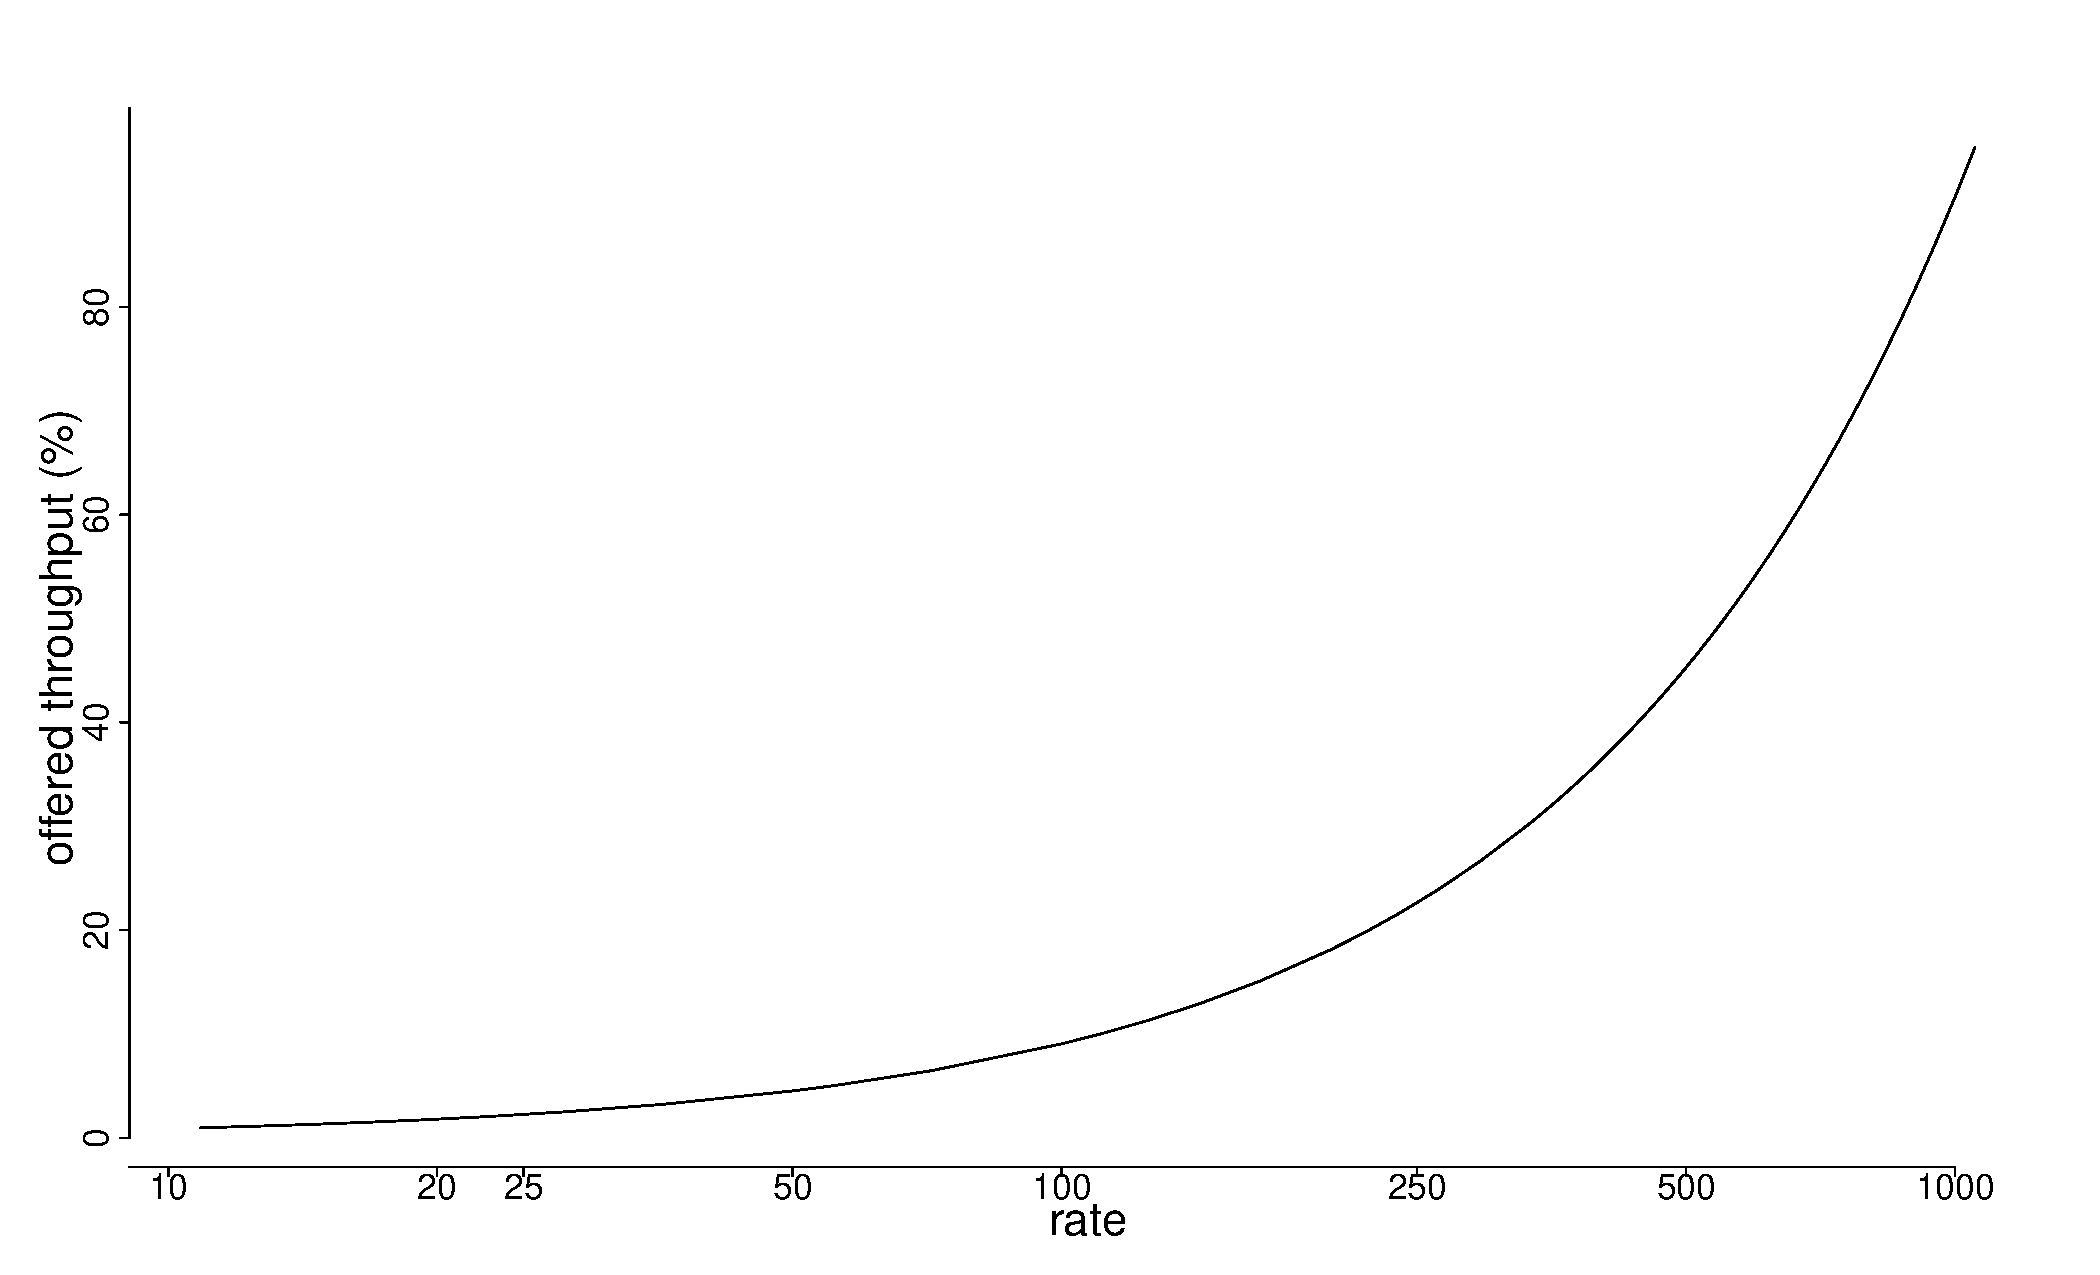
\includegraphics[width=\columnwidth]{graphs/Sim1}
    \caption{Relation between the free rate parameter (x logarithmic axis) and the offered throughput (y linear axis).}
    \label{grph:sim1}
\end{figure}

\begin{figure}[t]
    \centering
    \subfloat[Mean curve]{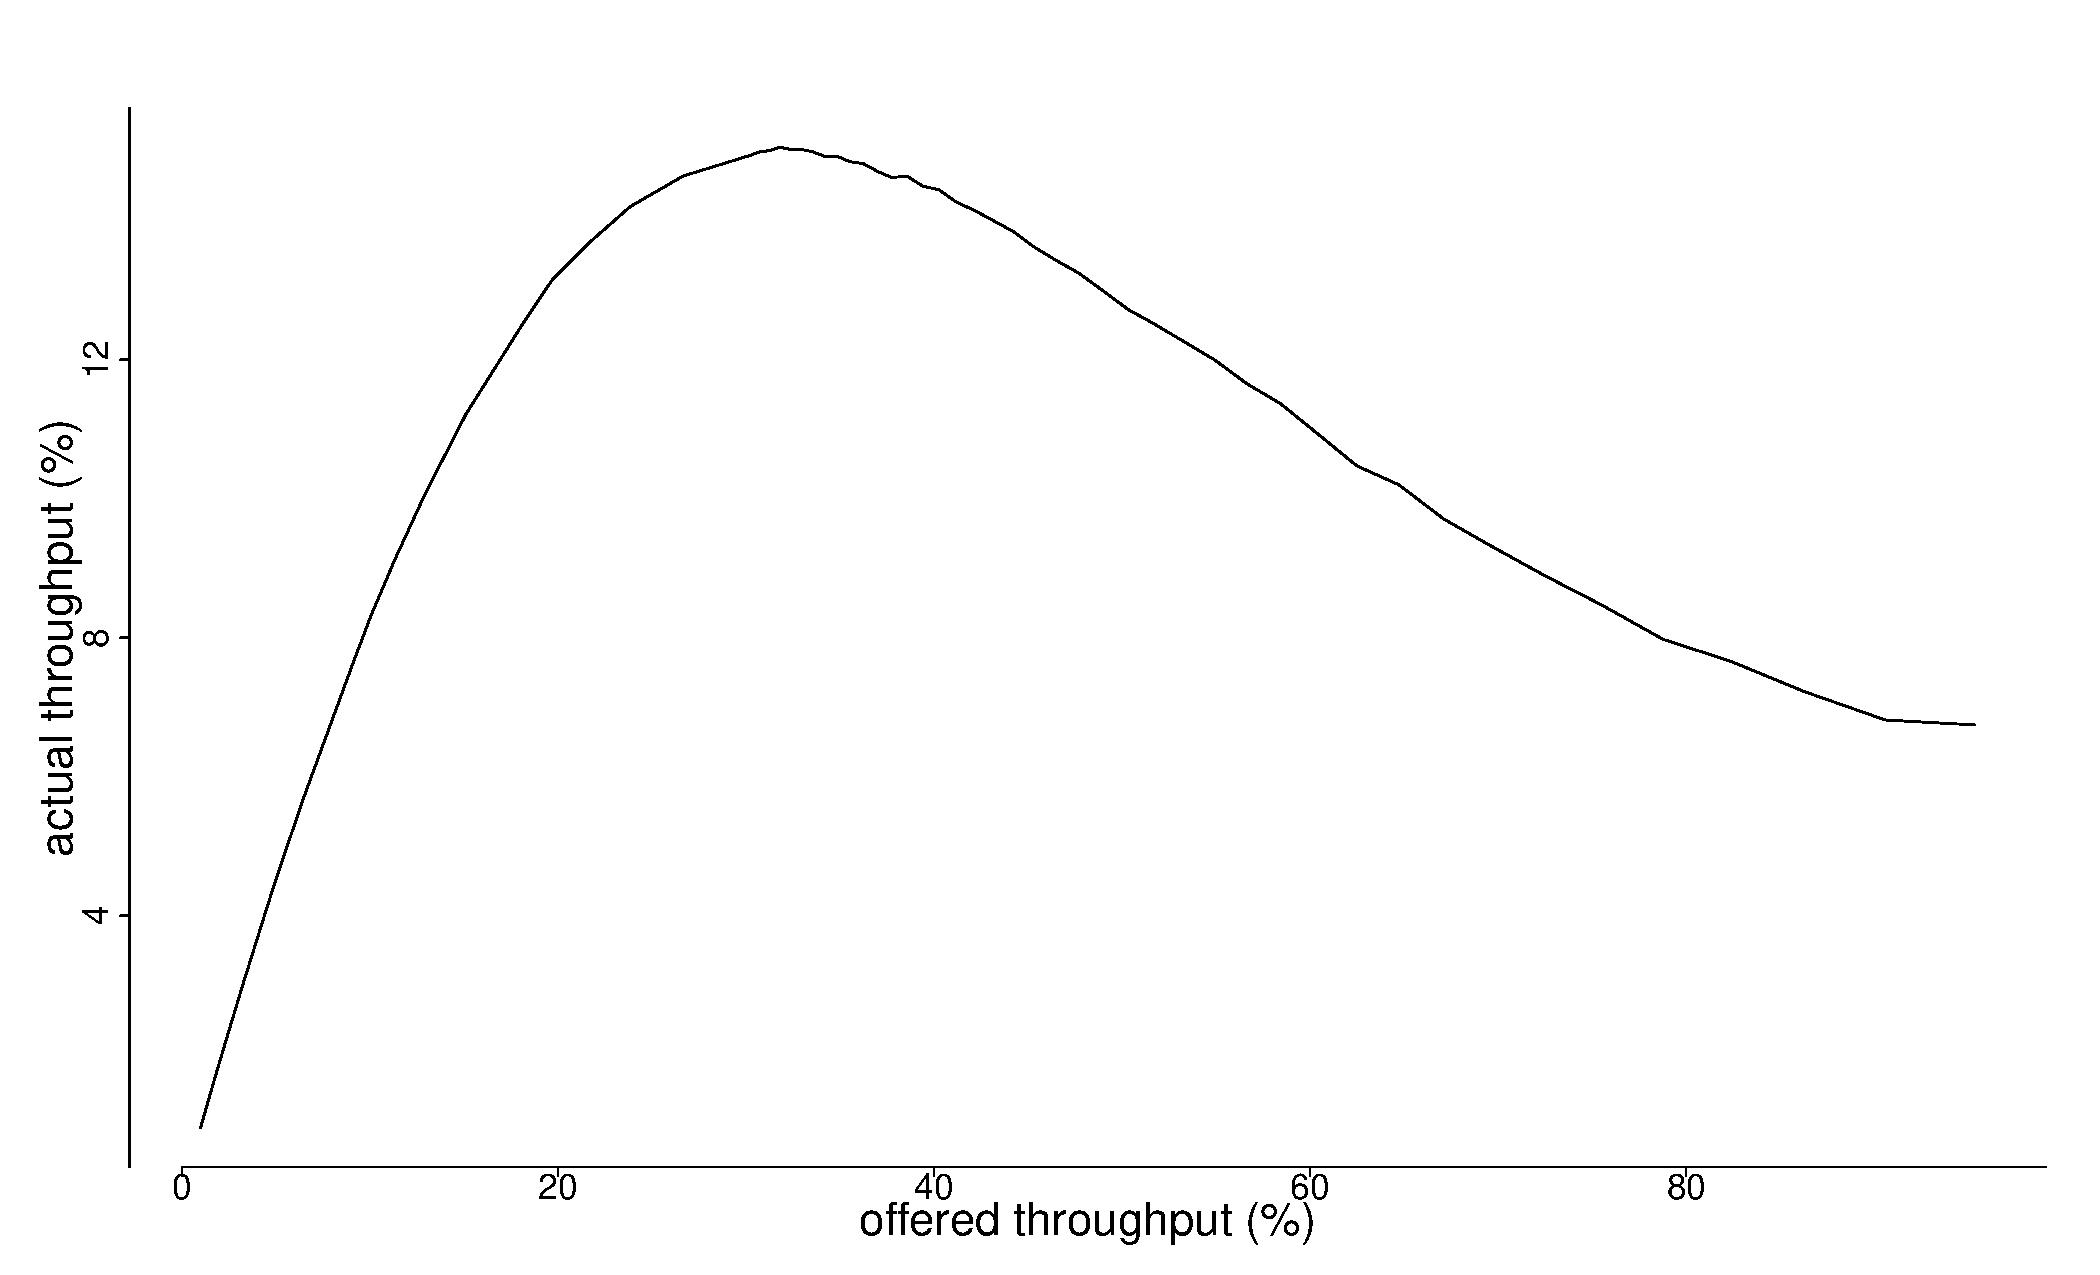
\includegraphics[width=\columnwidth]{graphs/Sim2}}\\
    \subfloat[Reliability boxes]{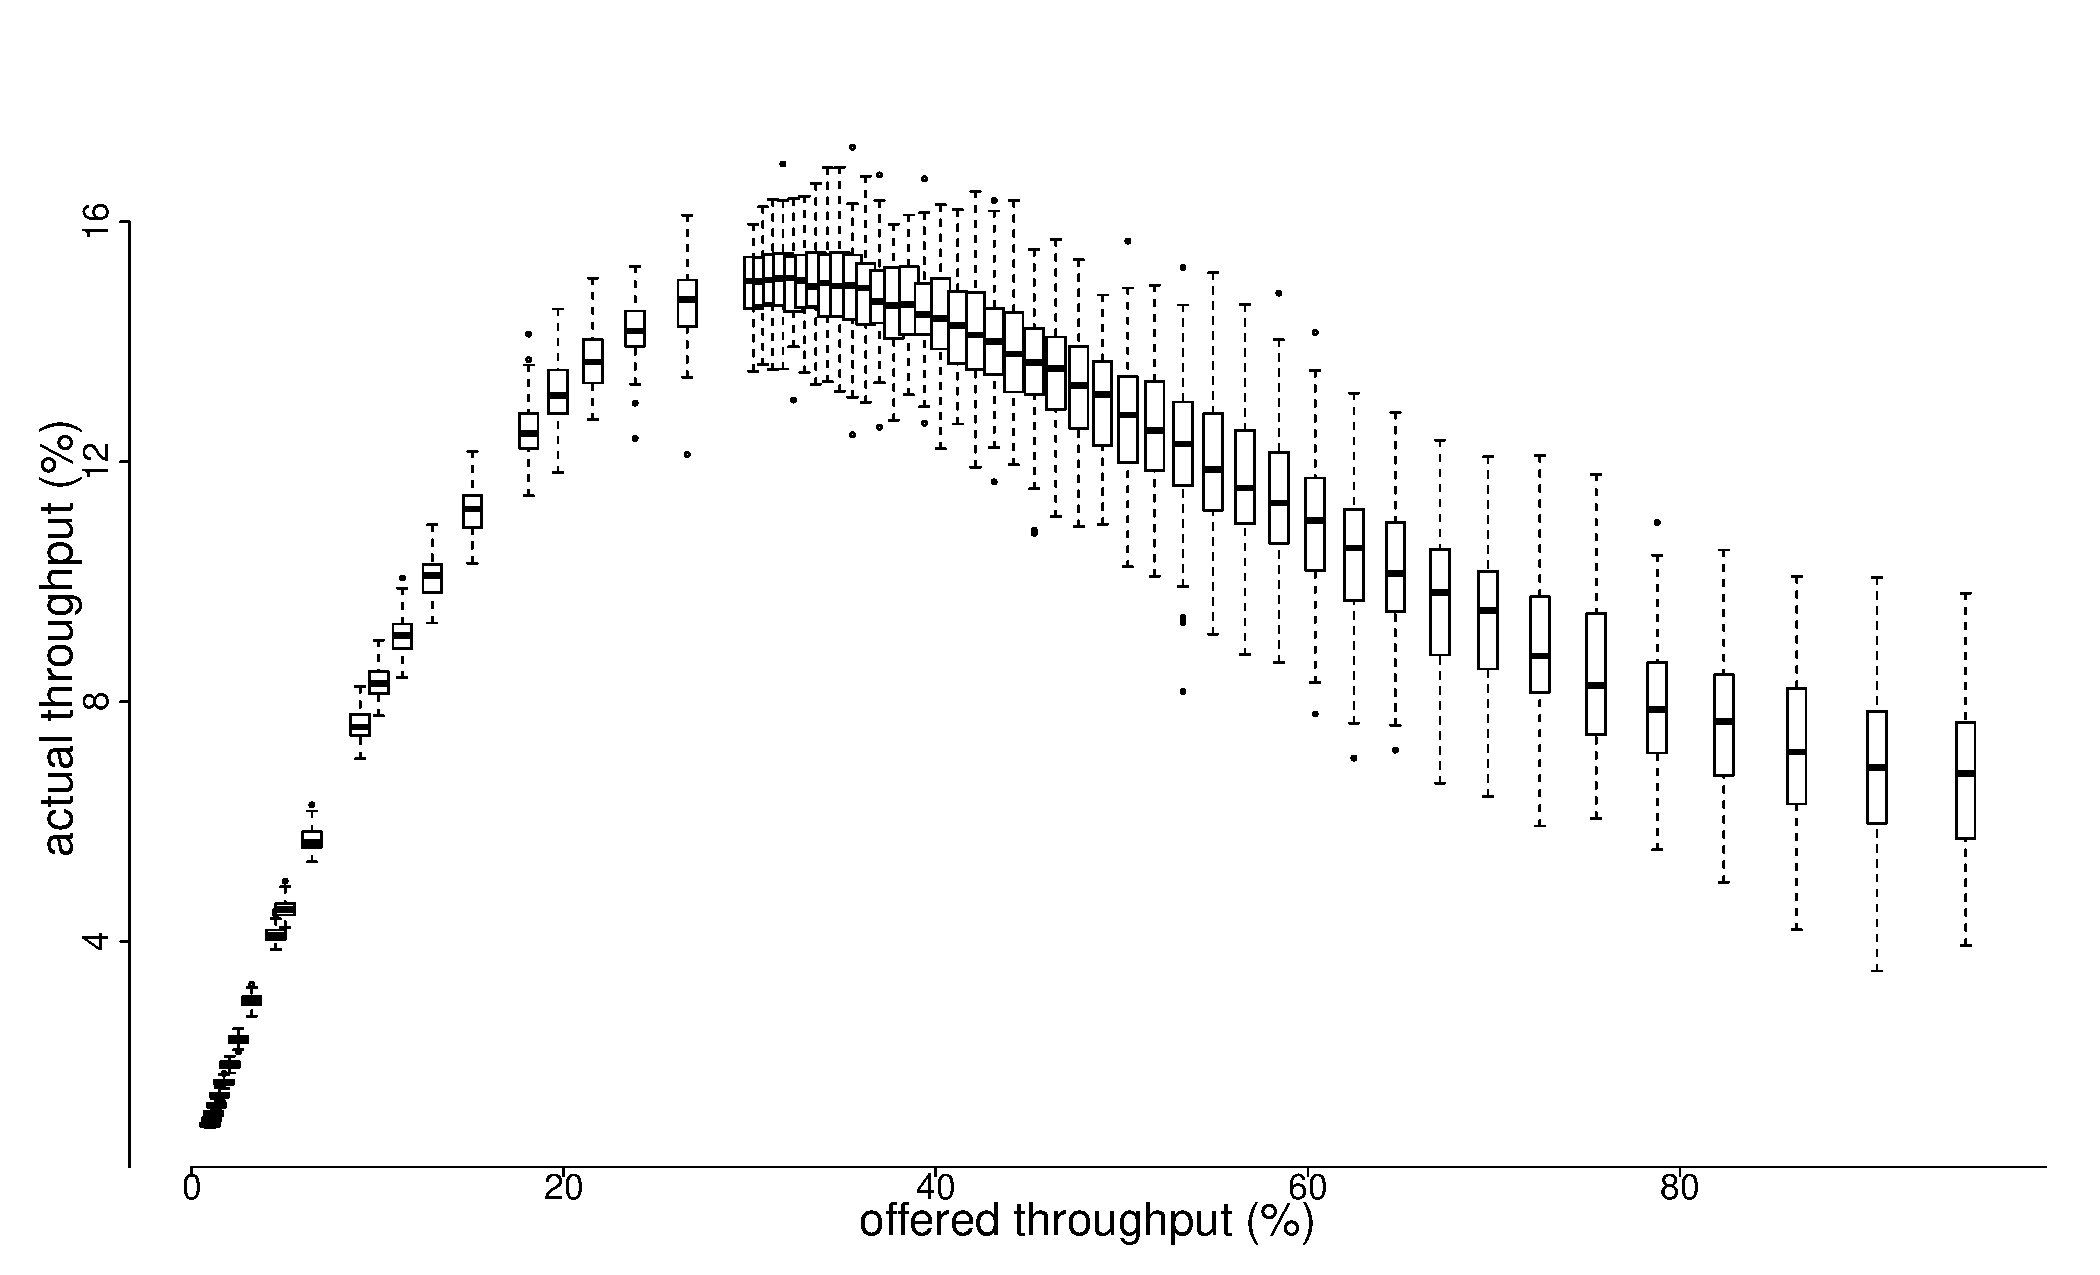
\includegraphics[width=\columnwidth]{graphs/Sim4}}
    \caption{Actual offered throughput varying the load of the network. Whiskers represents data’s reliability. The boxes’ upper and lower borders represent the 1st and 3rd distribution quartiles, the limits represent the whole distribution, and any additional dots are probable outliers.}
    \label{grph:sim24}
\end{figure}

\begin{figure}[t]
    \centering
    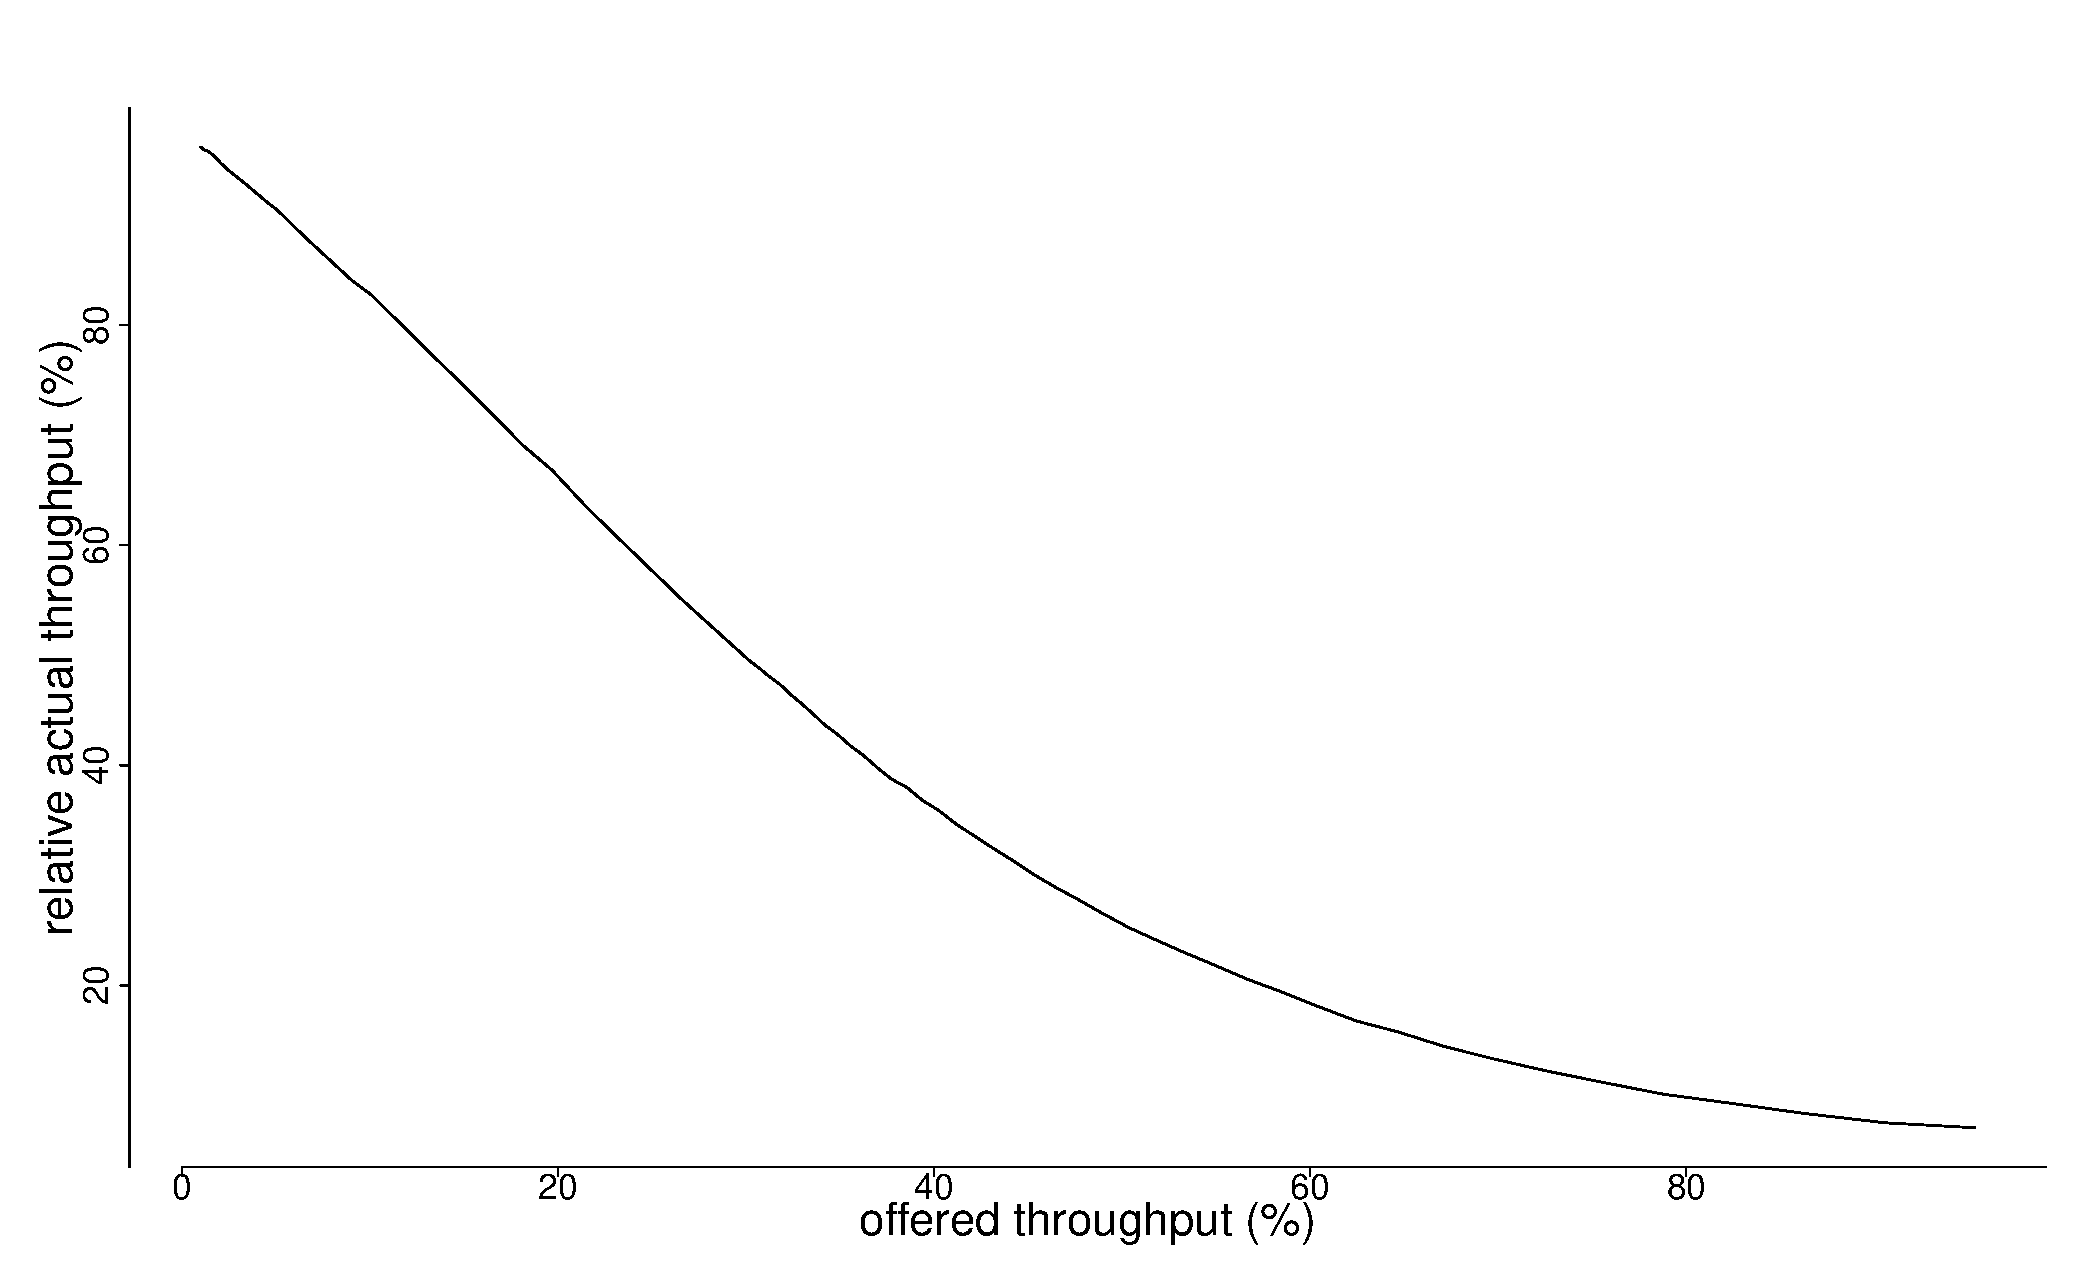
\includegraphics[width=\columnwidth]{graphs/Sim3}
    \caption{Actual offered throughput relative to the network throughput}
    \label{grph:sim3}
\end{figure}

\begin{figure}[t]
    \centering
    \subfloat[Mean curve]{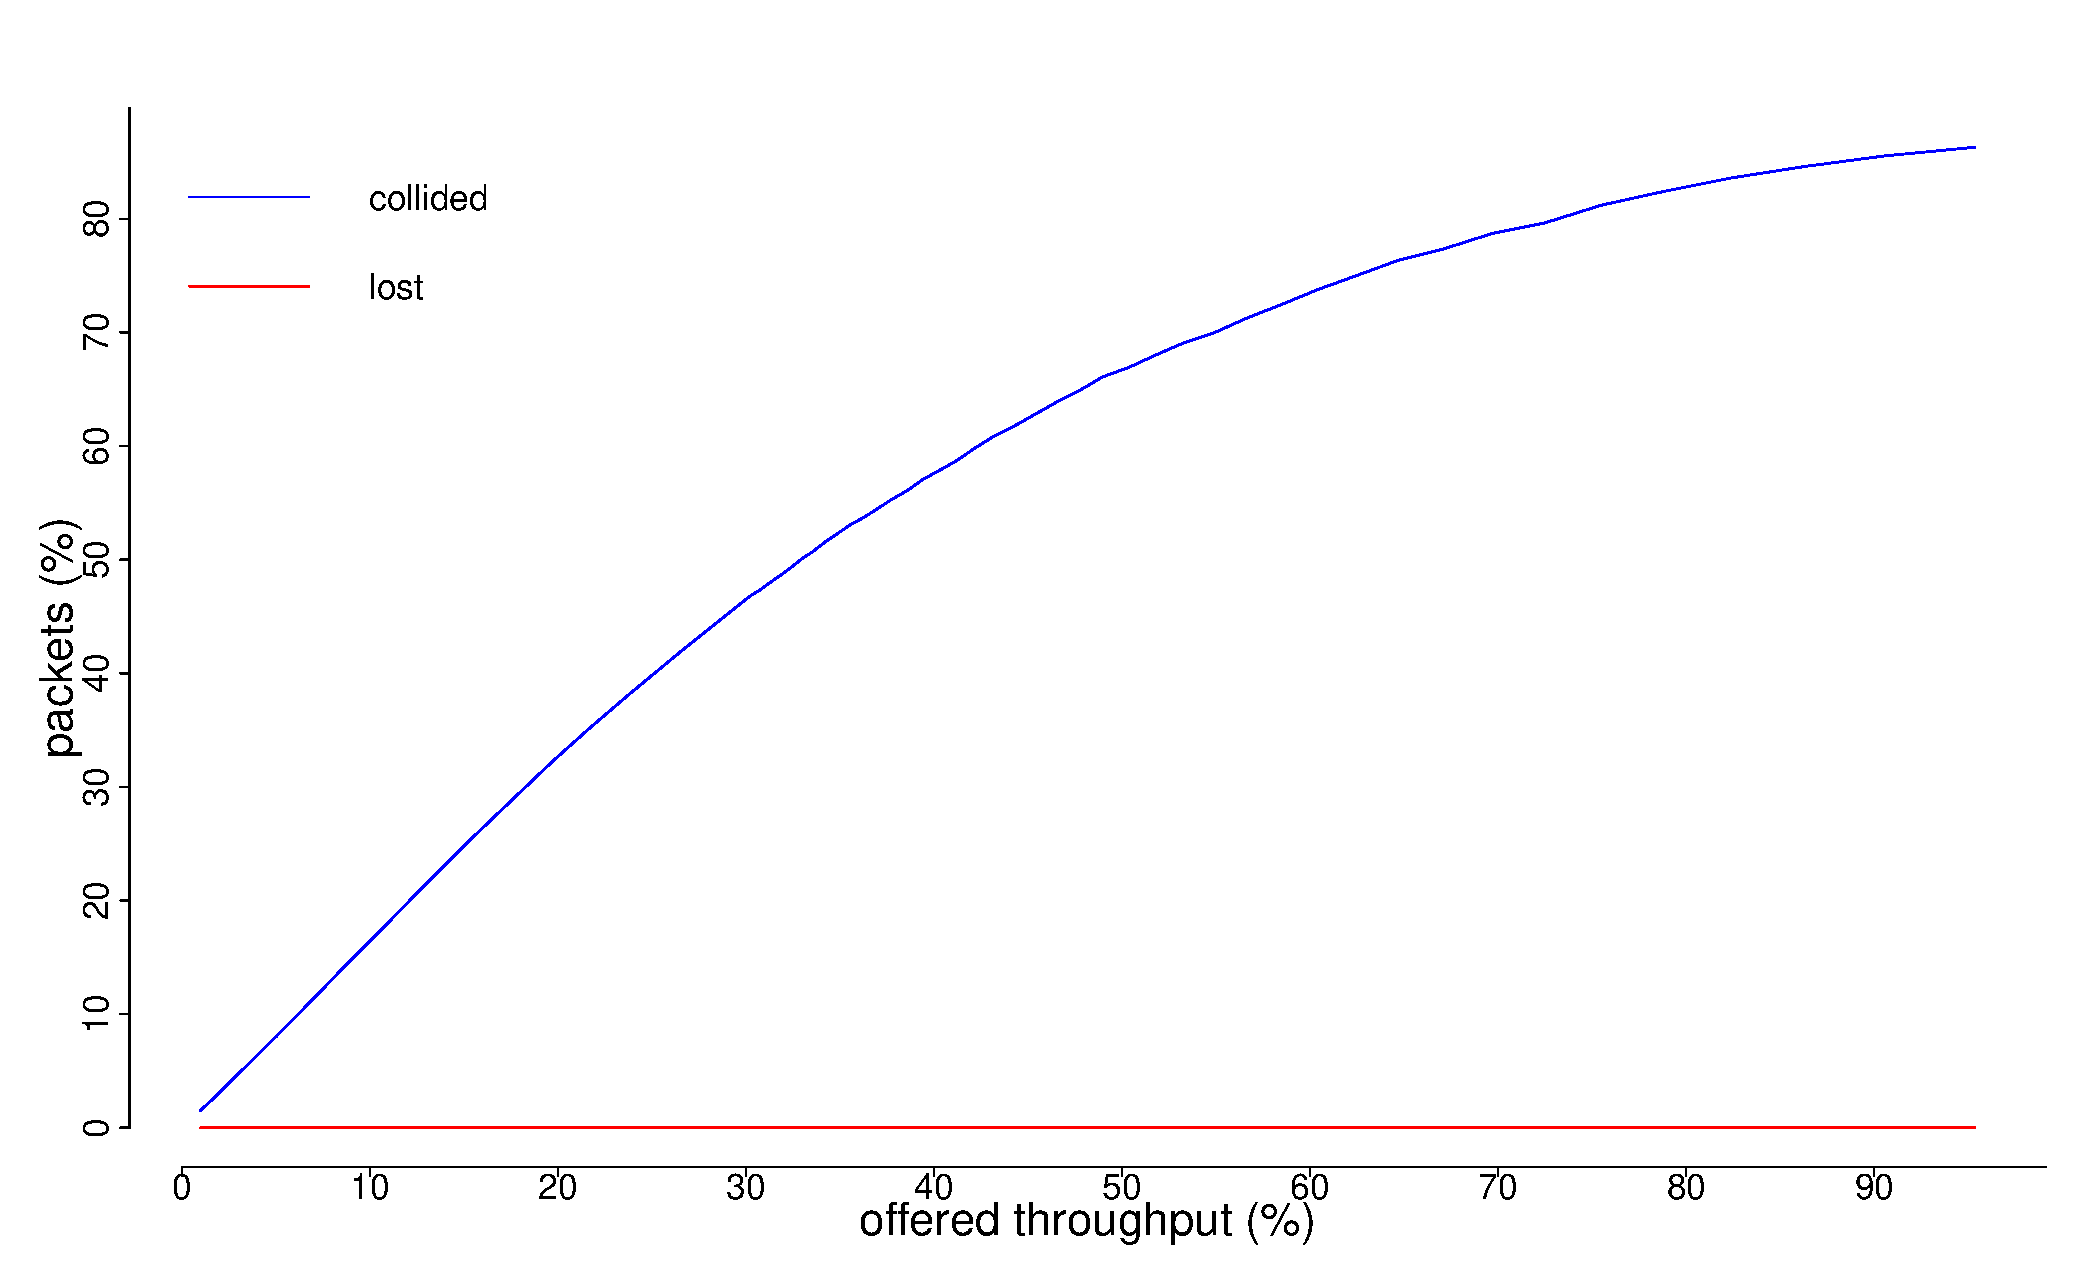
\includegraphics[width=\columnwidth]{graphs/Sim5}}\\
    \subfloat[Reliability boxes]{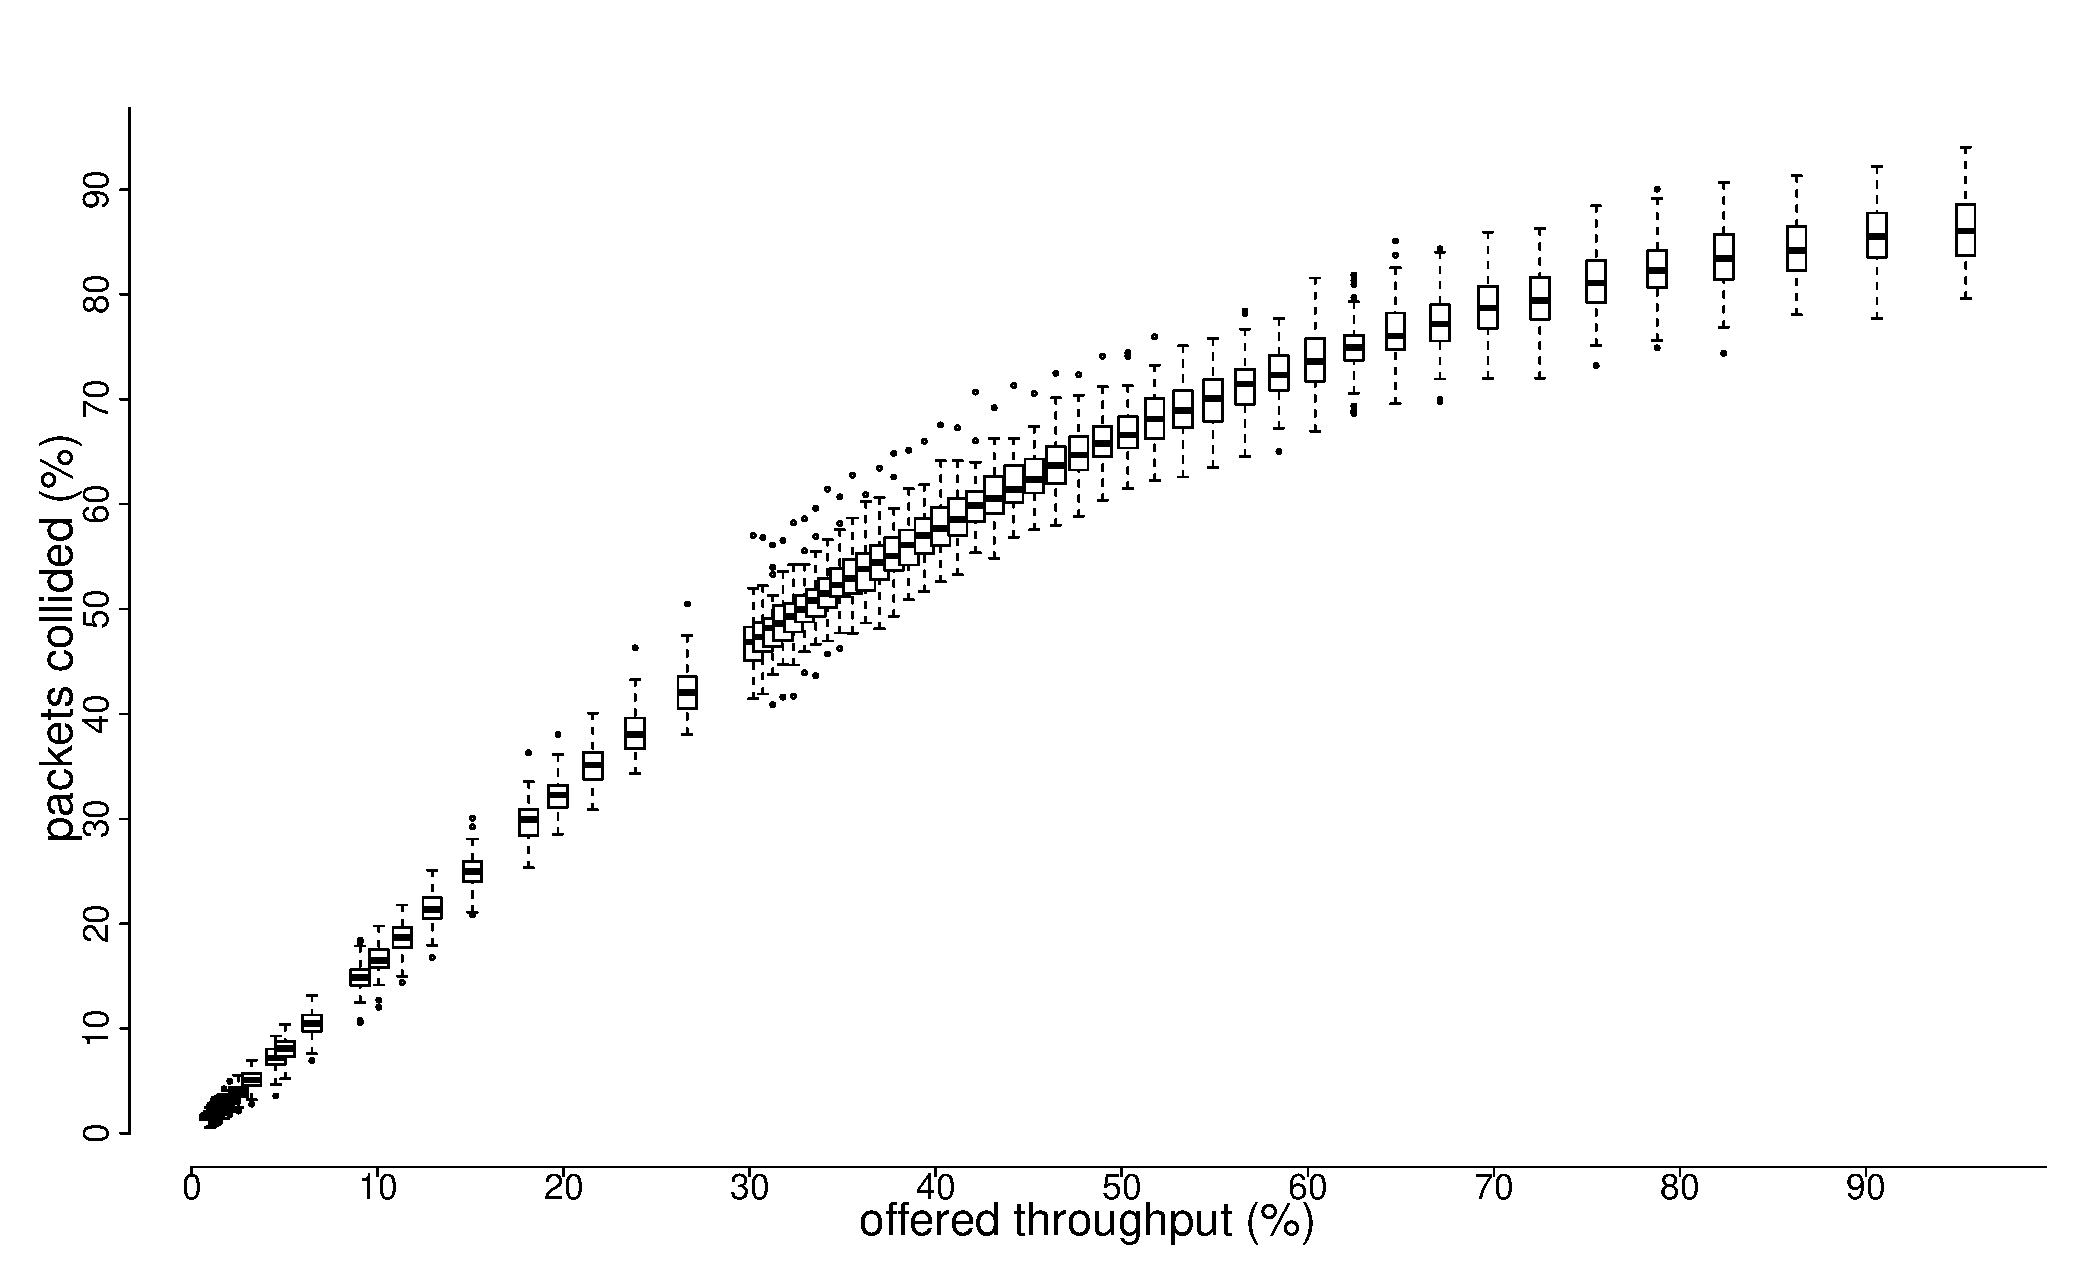
\includegraphics[width=\columnwidth]{graphs/Sim6}}
    \caption{Collided and lost packets varying the network load}
    \label{grph:sim56}
\end{figure}

\begin{figure}[t]
    \centering
    \subfloat[Mean curve]{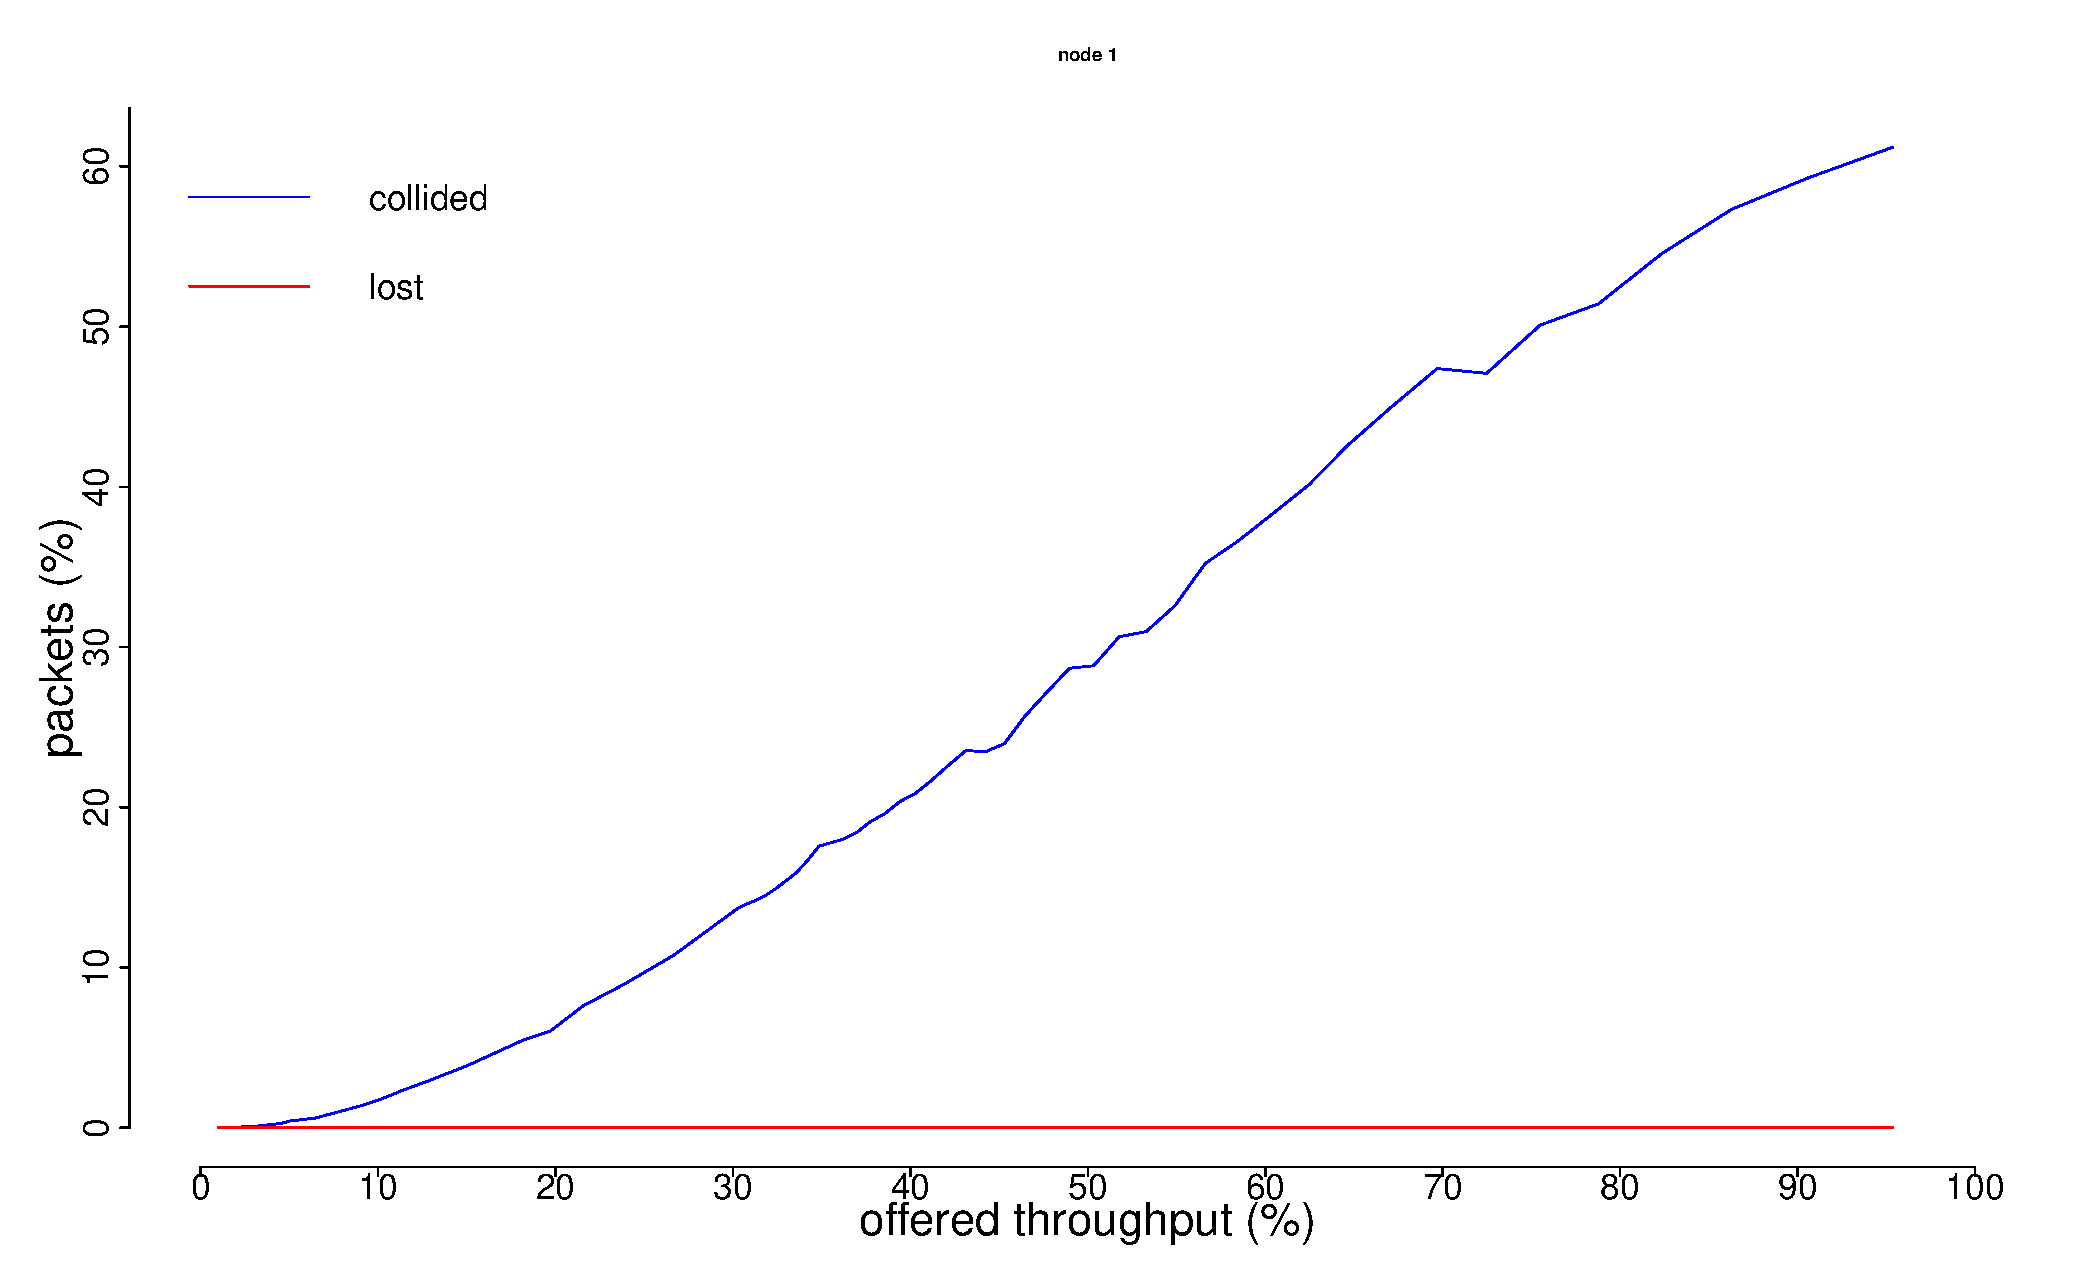
\includegraphics[width=\columnwidth]{graphs/Node1}}\\
    \subfloat[Reliability boxes]{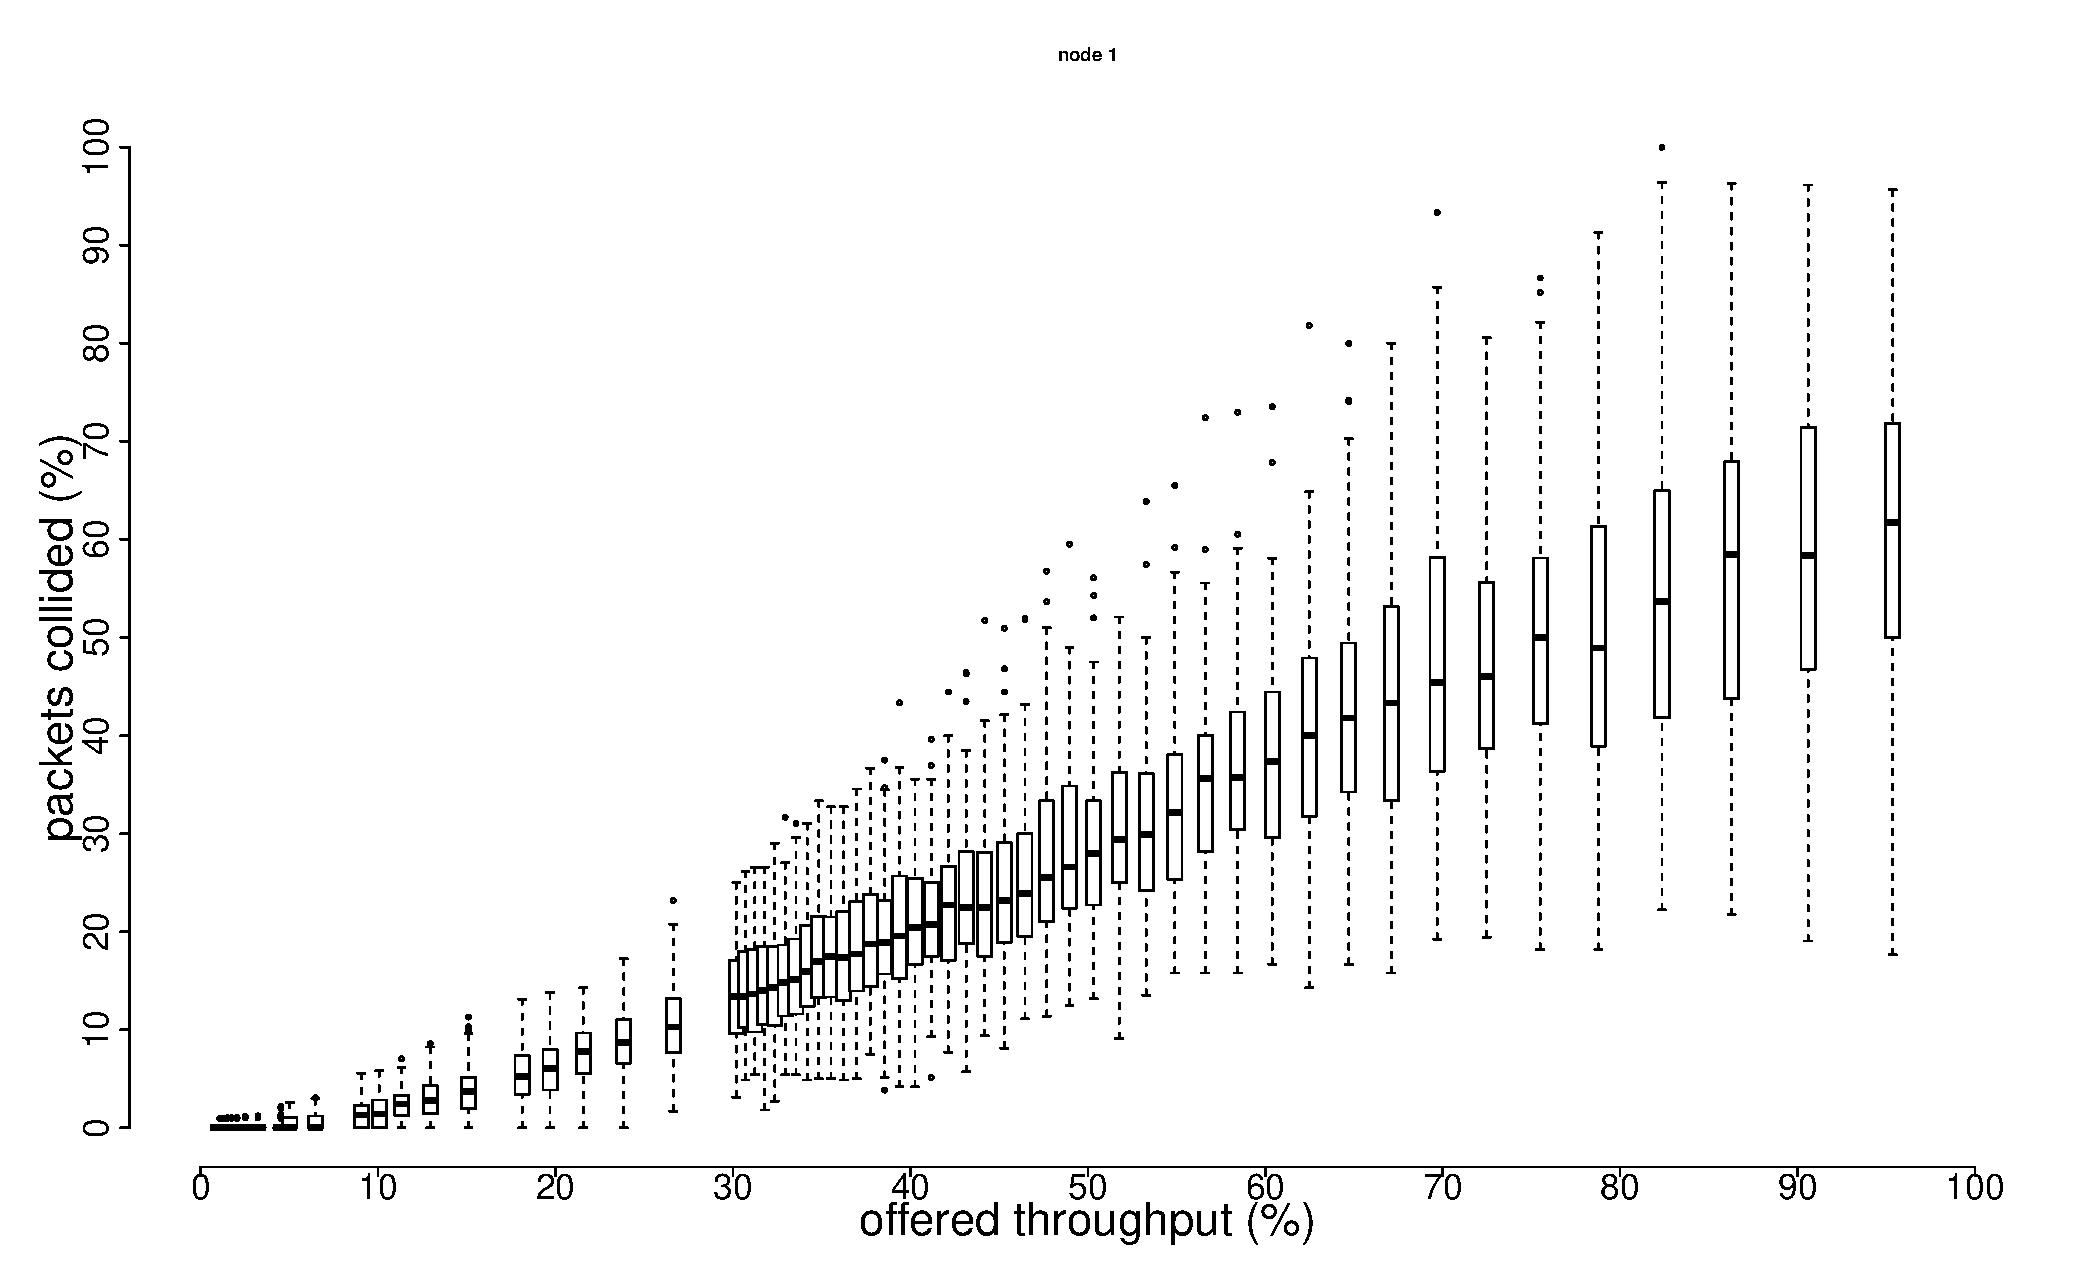
\includegraphics[width=\columnwidth]{graphs/Node1Boxplot}}
    \caption{Collided and lost packets in Node 1 varying the network load}
    \label{grph:node1}
\end{figure}

\begin{figure}[t]
    \centering
    \subfloat[Mean curve]{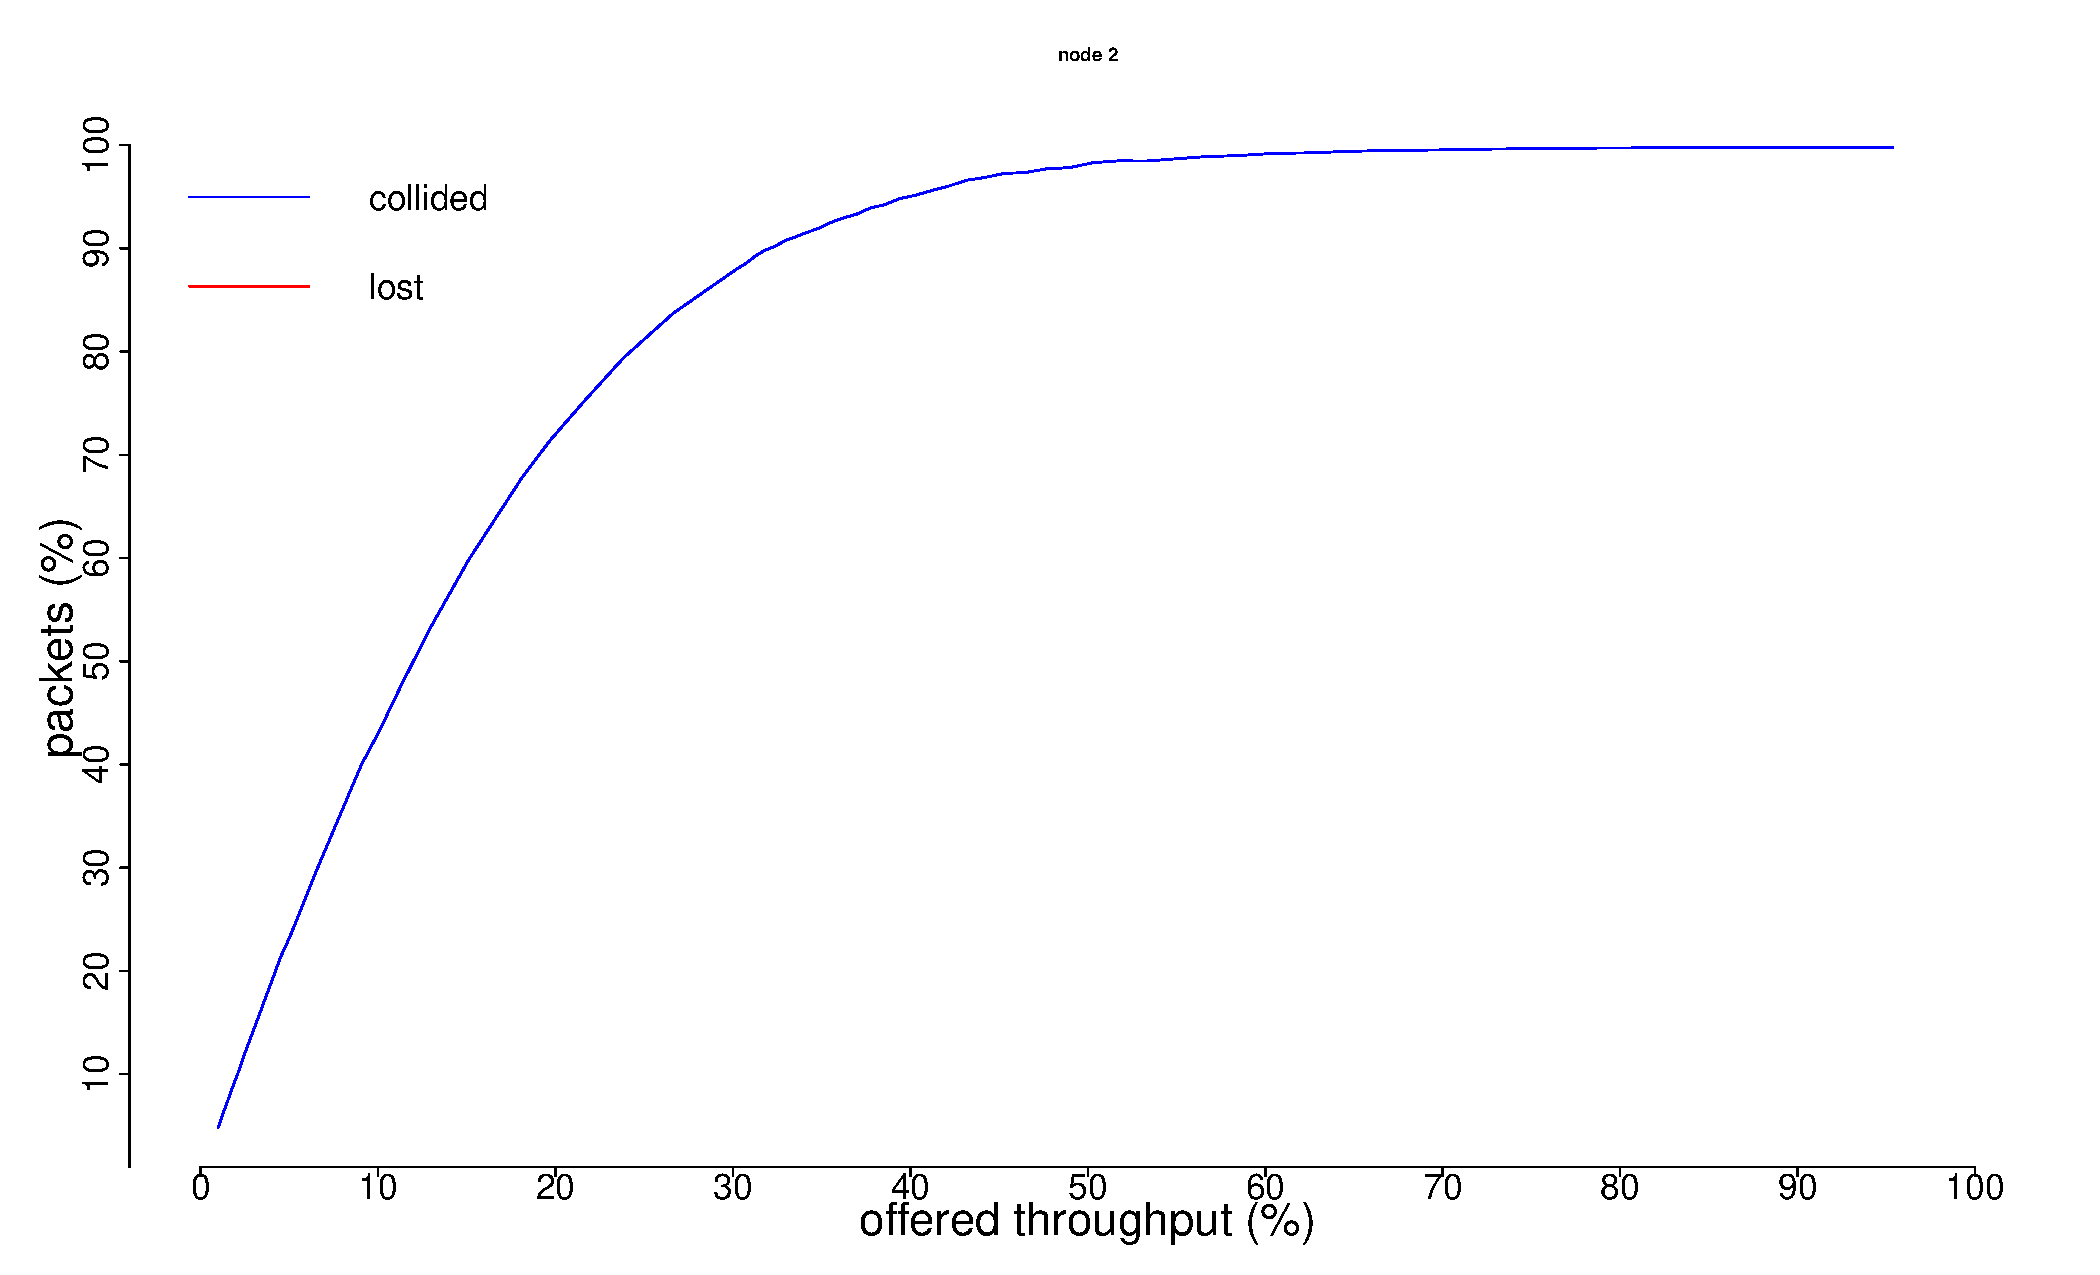
\includegraphics[width=\columnwidth]{graphs/Node2}}\\
    \subfloat[Reliability boxes]{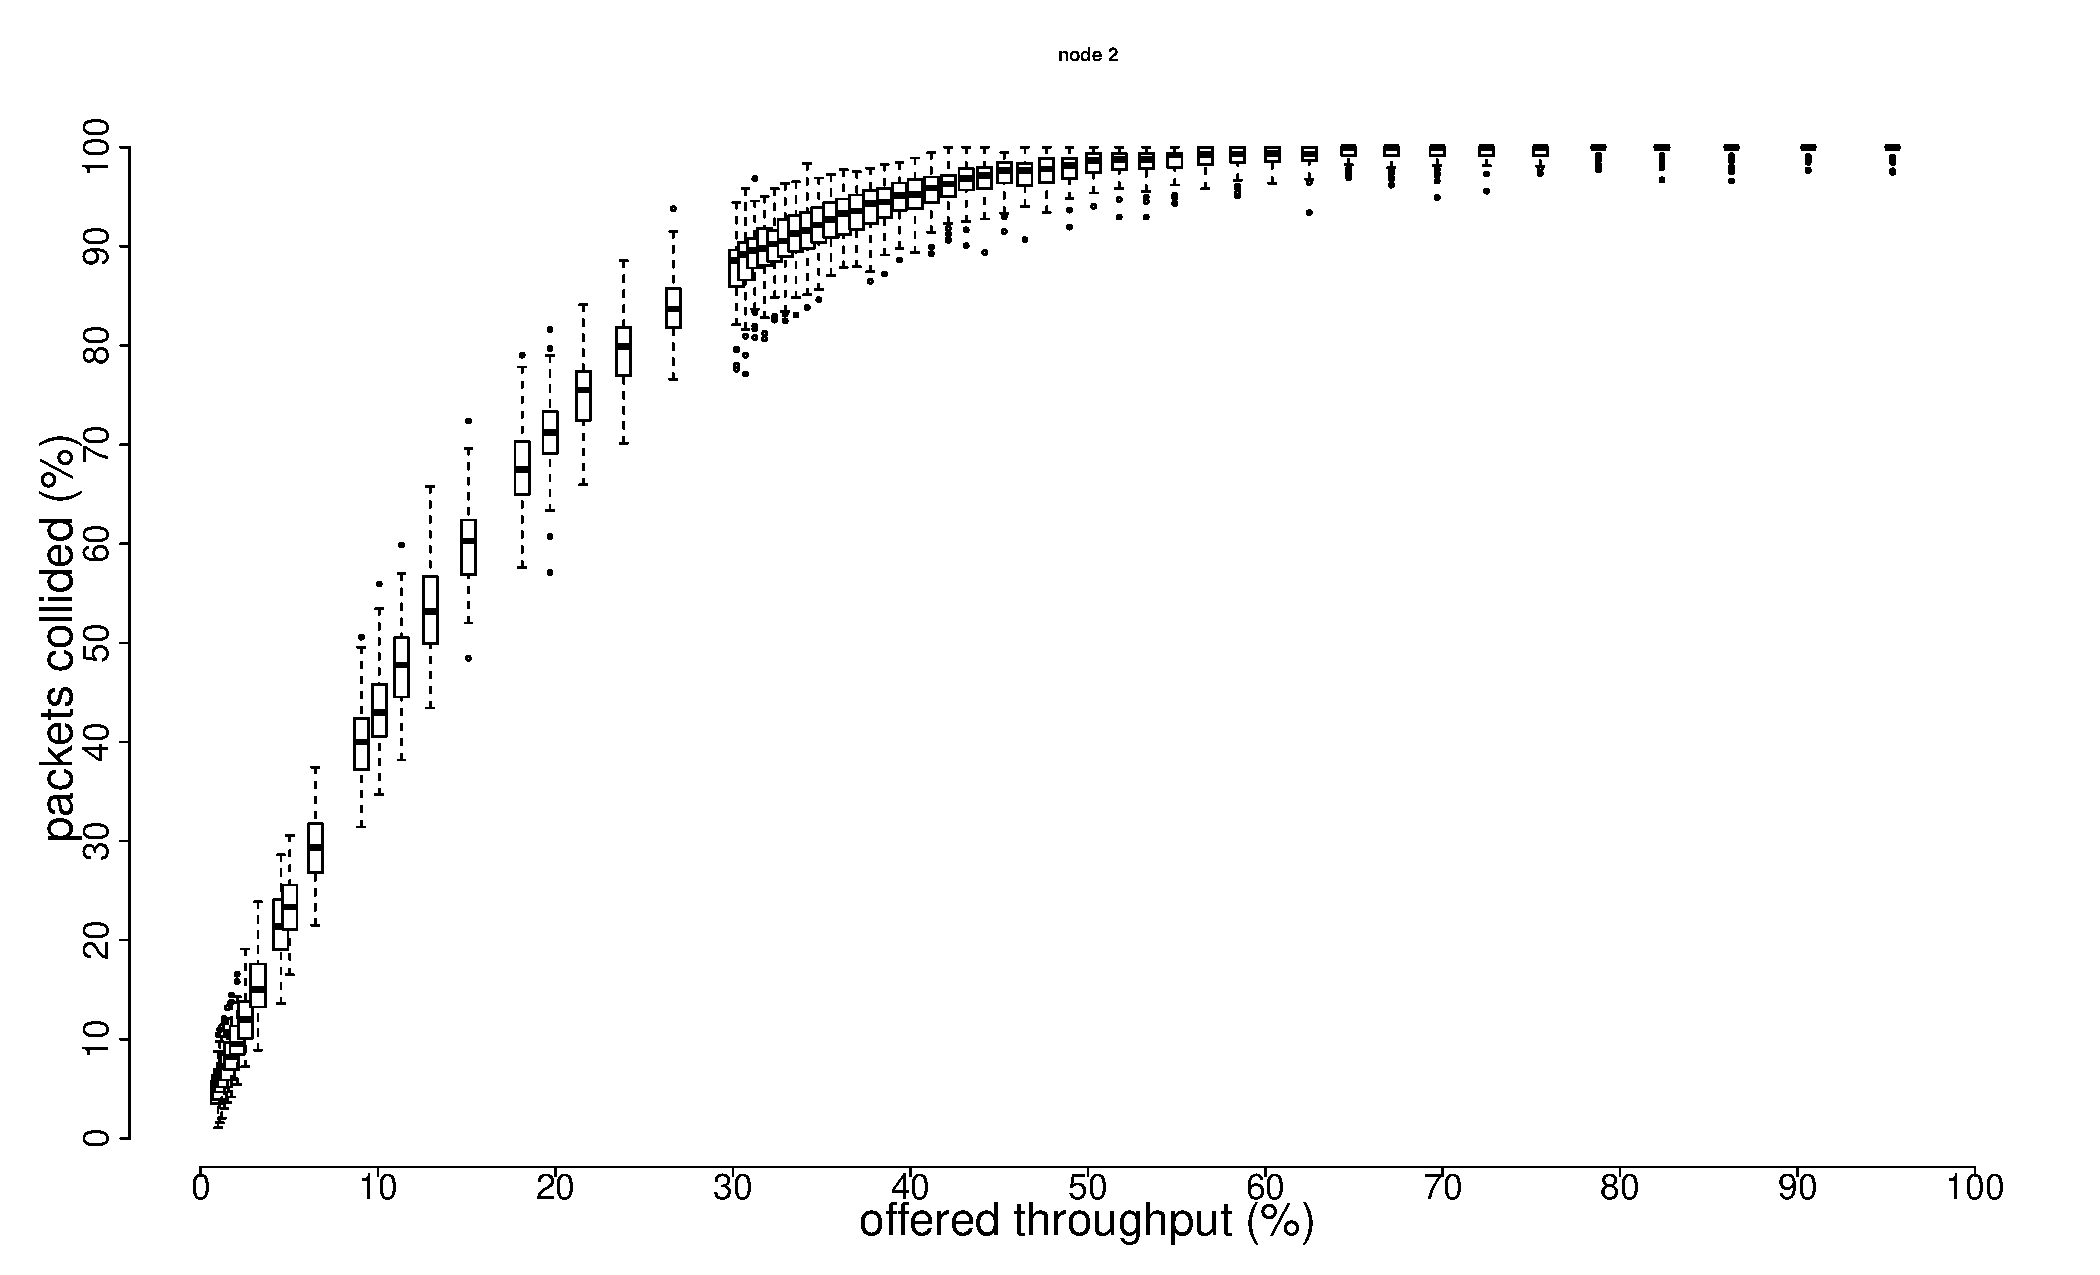
\includegraphics[width=\columnwidth]{graphs/Node2Boxplot}}
    \caption{Collided and lost packets in Node 2 varying the network load}
    \label{grph:node2}
\end{figure}

\subsection{Data analysis}\label{sec:dataanalysis}
\cref{grph:sim1} shows the direct correlation between the tunable rate parameter and the offered throughput of the network. The network works at its full potential when the rate parameter is around \(1000\); on the opposite, if the rate parameter is below \(10\) the network nodes are basically always idle (giving no interest in studying the net in that particular condition). To understand when the network performs better, the actual throughput, which does not take in consideration collided and lost packets, was calculated against the offered throughput, showing in \cref{grph:sim24} that when the network performs at \(30\%\) of its potential the successfully transmitted traffic is \(15\%\). On the other hand, while the network starts being saturated the actual percentage of successfully transmitted traffic drops to around \(6\%\). \cref{grph:sim3} shows the actual throughput relative to the actually-sent throughput, showing that when the network performs at low-levels of offered throughput the traffic is mainly successful with few collisions while when the net is under heavy load the traffic tends to be only composed by collided packets. \cref{grph:sim56} shows the percentage of collided and lost packets varying the load of the network, showing that when the traffic is maximized the number of collided packets is around \(85\%\). Looking again at \cref{grph:sim24} the maximum successful traffic achievable by the network is at \(30\%\) of full potential when a little less than \(50\%\) of the sent packets are collided and thus not usable anymore. To have different perspectives on how the internal network works two single nodes were studied, respectively the one with the most number of neighbors and the one with the least. Respectively Node \(2\) is the node with most neighbors (4) and from \cref{grph:node2} is clearly visible that the curve of packets collided over the offered throughput rise up quicker with respect to the system one shown in \cref{grph:sim56}, denoting that high clustered areas perform worse than the average system. On the other hand, low-density areas perform better as shown in \cref{grph:node1} which takes in consideration node \(1\) which has only 1 neighbor, that can send outgoing successful traffic with a higher rate with respect to the average of the system.

\section{Analytical model}\label{sec:analiticalmodel}

\subsection{Constraints}\label{sec:constraints}
A simplistic analytical model was devised from the given hard constraints in order to study it against the simulator. Several simplifications were used such that all the nodes are participating on the same channel thus broadcasting to every other node, the waiting queue of nodes is removed and the packets size is always the same across all transmissions for every node. 

\begin{figure}[t]
    \centering
    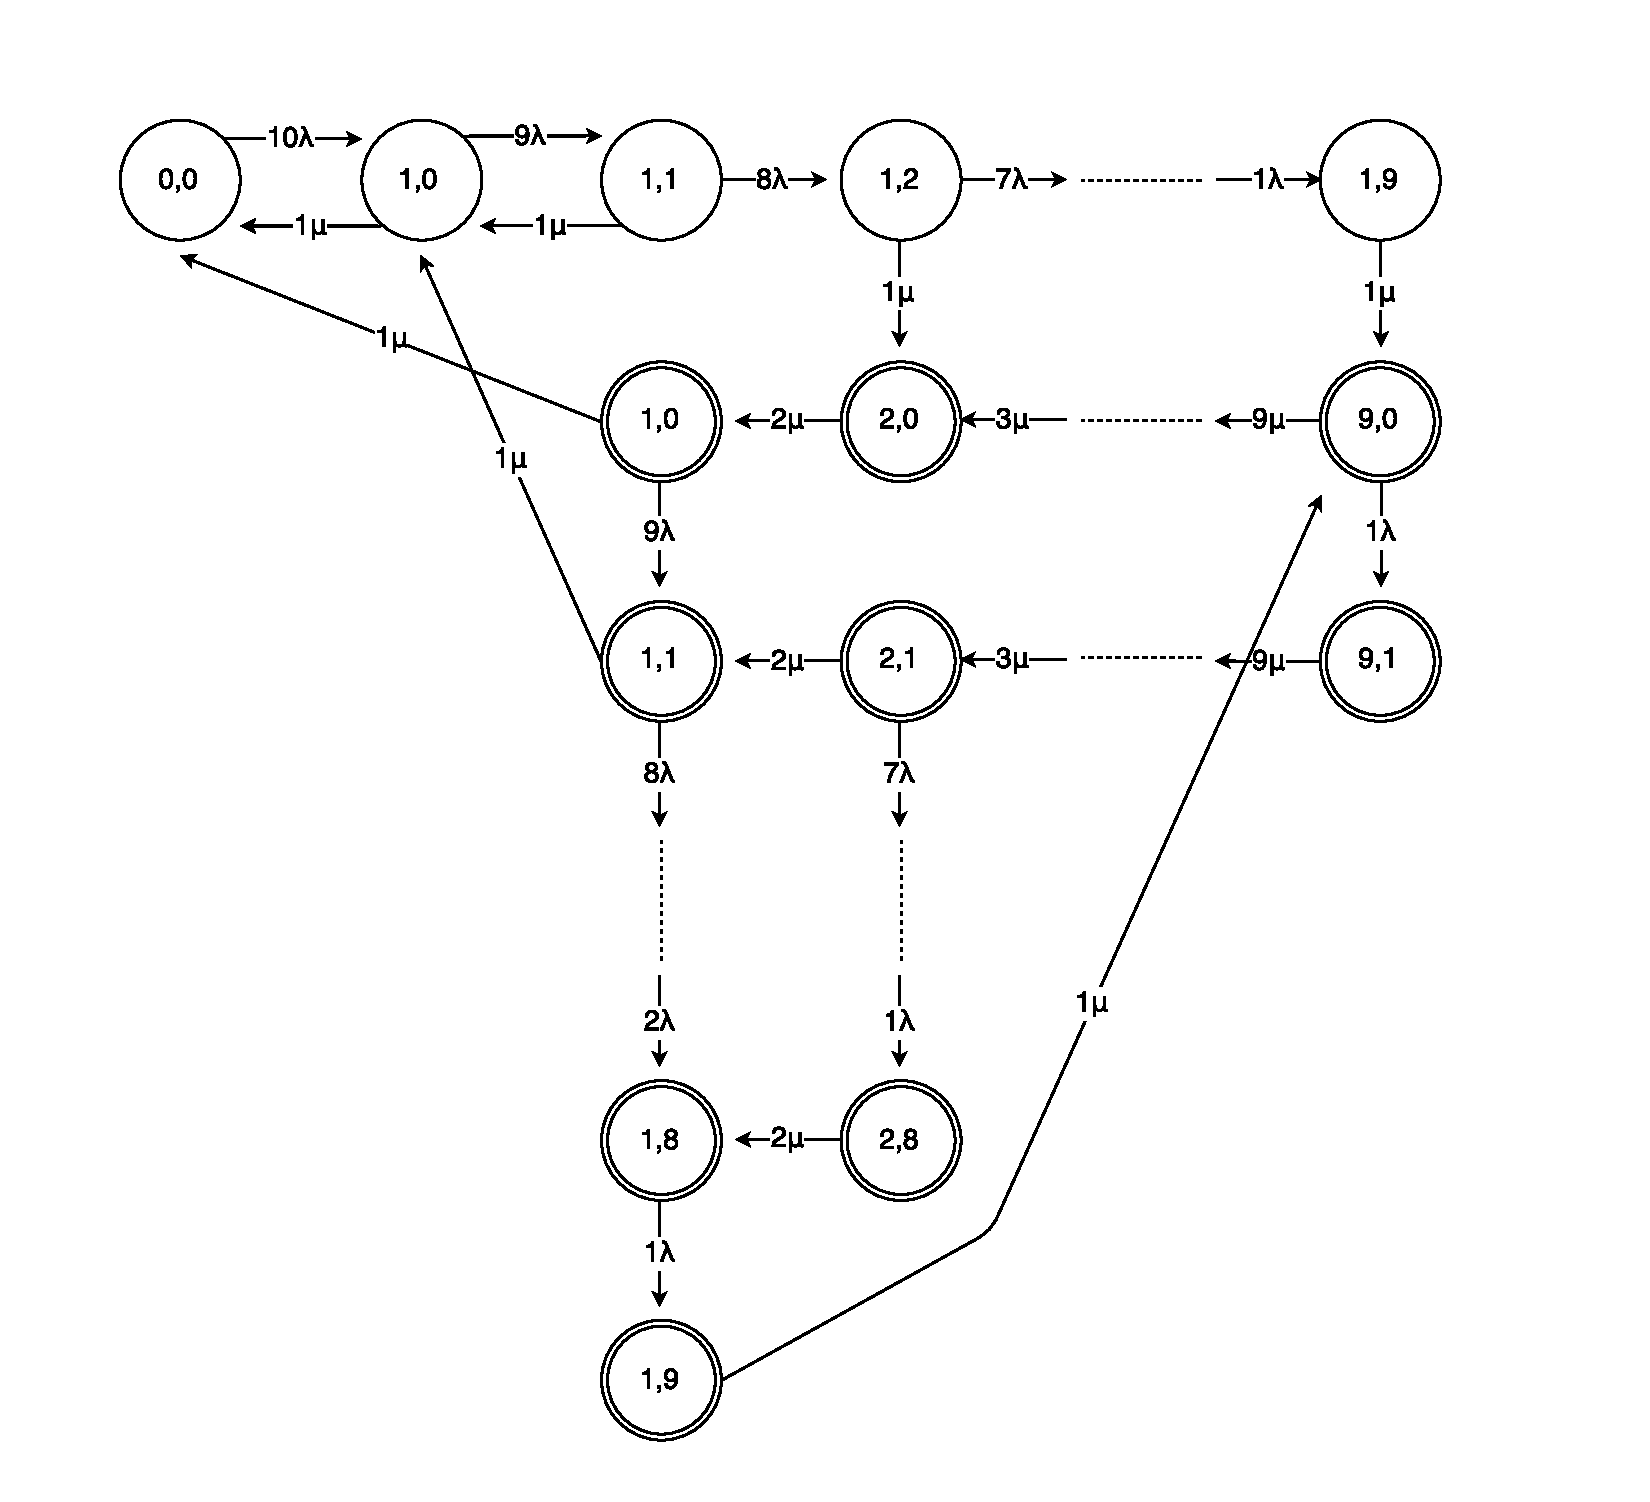
\includegraphics[width=\columnwidth]{graphs/MCTS}
    \caption{One time circled states mark no collisions, twice circled states mark collisions and inside the circles, there is a tuple representing the number of nodes transmitting \(Nt\) and the number of nodes waiting to transmit\(Nw\)}
    \label{fig:mcts}
\end{figure}

\subsection{Model}\label{sec:model}
A Continuous Time Markov Chain was used to devise the model, in particular, it was used the infinitesimal generator represented in \cref{eq:infinitesimalgenerator} where \(q_{ij}\) are the rate of transitions from the state \(i\) to state \(j\) and state \(q_i\) is given by the \cref{eq:qi}.

\begin{equation}
    Q=[q_{i,j}]=\begin{Bmatrix} q_{0} & q_{0,1} & \cdots \\ q_{1,0} & q_{1} & \cdots \\ \vdots & \vdots & \ddots \end{Bmatrix}\label{eq:infinitesimalgenerator}
\end{equation}

\begin{equation}
    q_i=-\sum_{j=0,j\neq i}^{\infty}q_{ij}\label{eq:qi}
\end{equation}

It must be stated that state transitions could occur at any time, and the time between transitions is exponentially distributed. Exploiting the memorylessness of the exponential distribution, the future outcome of the process depends only on the present state. The steady-state probability vector \(\pi\) of the system was computed with \cref{eq:system} from the Markov Chain in order to have an insight on the average performances of the system when it stabilizes. The transition matrix Markov Chain used is represented in \cref{fig:mcts}.

\begin{equation}
    \left\{\begin{matrix} -\sum_{i=0}^{\infty}\pi_i=1 \\ \pi Q=0 \end{matrix}\right.\label{eq:system}
\end{equation}

Transitions across the Markov Chain are divided into two types: one associated with the end of a transmission and it is equal to the number of transmitting nodes multiplied by the rate \(\mu\), set to 1, the other type of transition is the generation by an idle node of a packet and it is equal to $ (10 - Nt - Nw)*\lambda $ which is equal to the idle nodes multiplied by the inter-arrival rate $ \lambda $, which is a free parameter and is variated between \(0.001\) and  \(0.1\) (in the simulator it was used the scale parameter which is just the inverse of the rate parameter).

\subsection{Implementation}\label{sec:implementationmodel}
The model was implemented in Python 3 language using the mathematical module Numpy for working with matrices. A matrix composed by the states represented in \cref{fig:mcts} is initially computed, then for each different rate parameter $ \lambda $ (ranging from \(0.001\) to \(0.1\)) a transition matrix (in the same format as \cref{eq:infinitesimalgenerator}) is derived and from it, the steady state matrix is computed and saved in a useful \(CSV\) format for the later analysis. The file generated by the Python script is then imported into the R script used to analyze the simulator in order to have both the data coming from the simulator and from the model.

\begin{figure}[t]
    \centering
    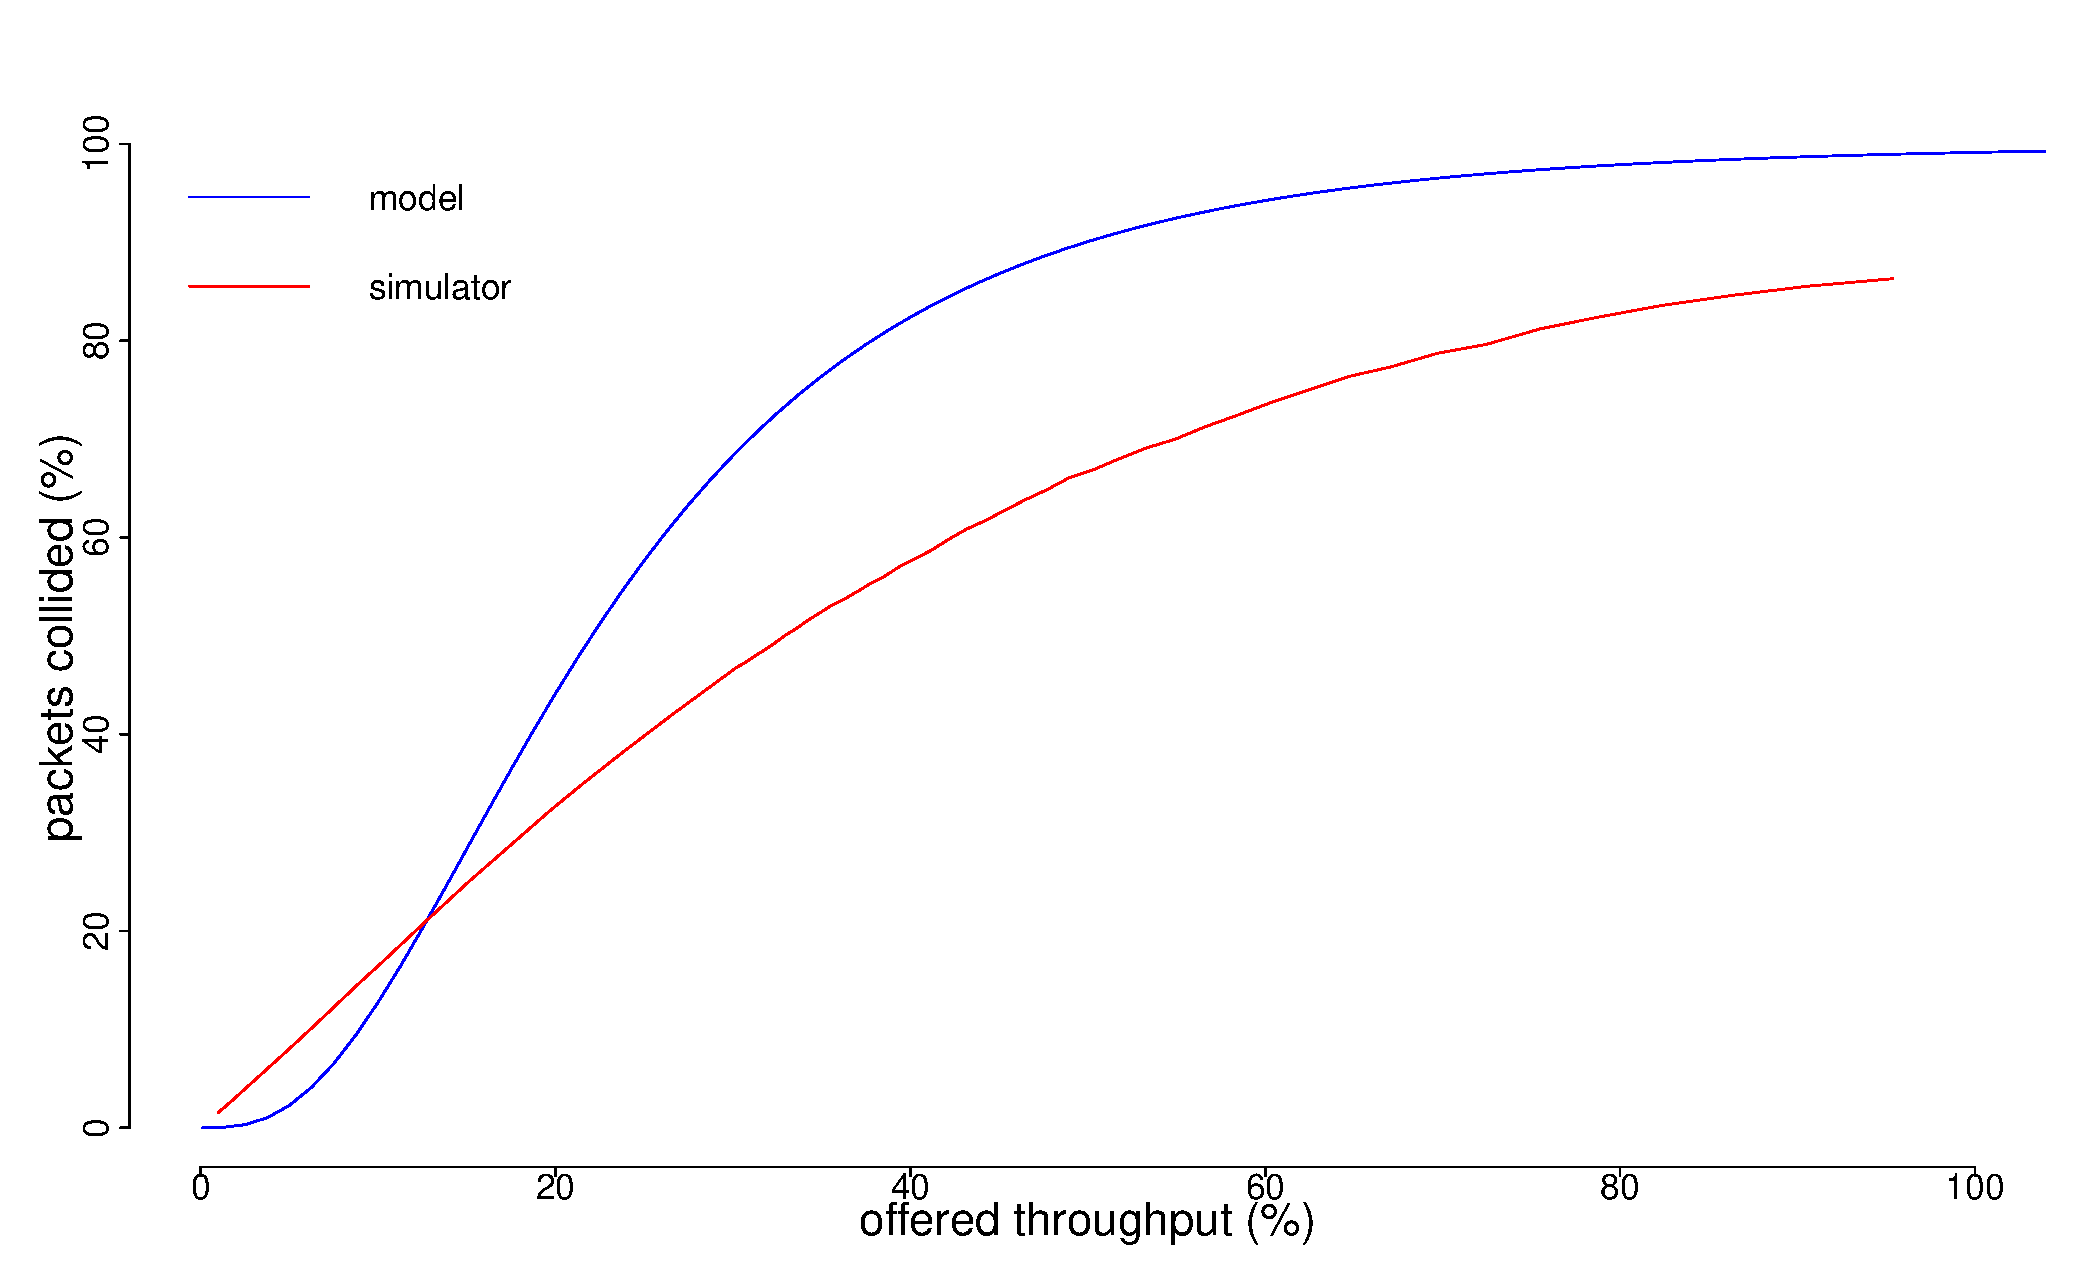
\includegraphics[width=\columnwidth]{graphs/Model1}
    \caption{Actual offered throughput of the model in blue, of the simulator in red, varying the network load}
    \label{grph:model1}
\end{figure}

\begin{figure}[t]
    \centering
    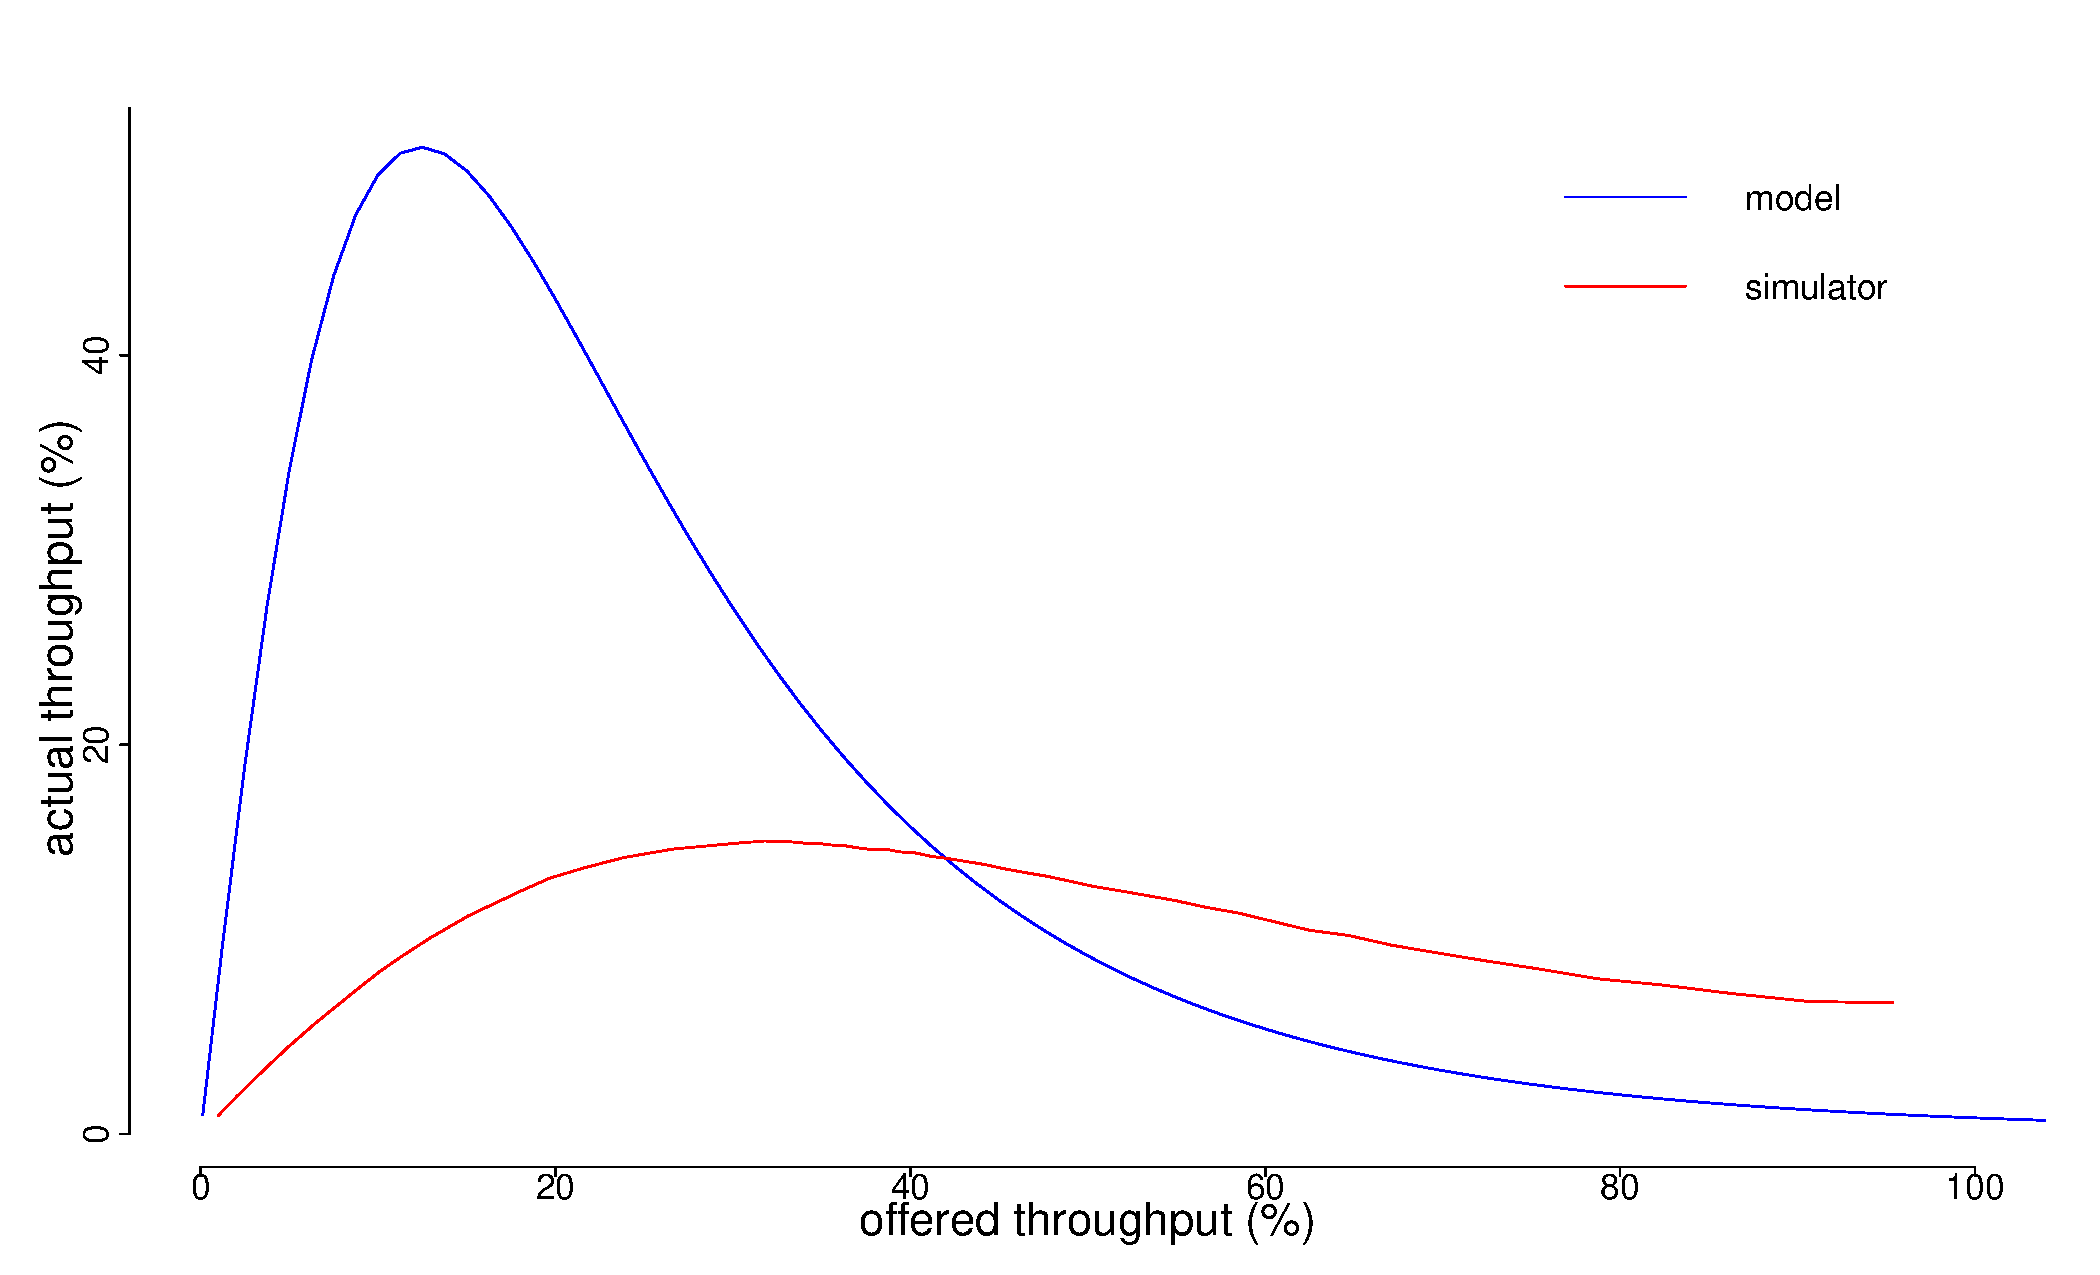
\includegraphics[width=\columnwidth]{graphs/Model2}
    \caption{Collision rate of the model in blue, of the simulator in red, varying the network load}
    \label{grph:model2}
\end{figure}

\subsection{Data Analysis}\label{sec:dataanalysismodel}
\cref{grph:model1} shows the comparison between the model and the simulator in terms of actually offered throughput over the network load in percentages. It is evident from the chart that the trend of the model and the simulator are similar, having the model performing better at lower transmission rates and the simulator performing slightly better at high loads. This difference of performances is due to the simplification made earlier on how the model was built since all the 10 nodes in the model can transmit with each other, thus when the load is small a packet generated by a node is received by all the ten nodes while in the simulator that packet could have been received by only the neighbors of the single node which in average are 2. The model, on the other hand, performs worser at high loads since all the ten nodes are clumped together, thus incrementing the collision rates. This claim is confirmed by \cref{grph:model2} which shows the packet's collision rate when the load of the network is increased. The model curve, in fact, reaches firstly, with respect to the simulator one, the point of full saturation when all the packets in the network collide. 

\subsection{Pure ALOHA comparison}\label{sec:purealohacomparison}
It is natural to compare the model designed with the Pure ALOHA protocol. Pure ALOHA protocol can be summarized in the \href{https://en.wikipedia.org/wiki/ALOHAnet#Pure_ALOHA}{two following bullet points}
\begin{itemize}
\item If you have data to send, send the data.
\item If, while you are transmitting data, you receive any data from another station, there has been a message collision. All transmitting stations will need to try resending "later".
\end{itemize}
It is clearly visible that Pure ALOHA and the model discussed are similar but some profound difference are present. Pure ALOHA protocol lacks any carrier sensing technique and thus if a packet has to be sent it will be sent even if the network channel is busy while the discussed model will transmit packets only when the network is free. The discussed model, moreover, will transmit any packet (just generated, waiting or in the queue) as soon as the network will become free without any back-off strategy, strategy which is instead present in the Pure ALOHA protocol although with no specific implementation. In the end, these two models appear behaving similarly.

\section{Conclusion}\label{sec:conclusion}
Two approaches to evaluating a possible-real network system were presented. The first one simulated the network programmatically with one free parameter which was the inter-arrival time of packets which ruled the load of the network. Knowing how the network performs with different kinds of traffic is indeed essential for the latter decision of where, when and for how much time to use this type of network. The second approach to study the network was done analytically by devising a simplified model of the real network and then solving it finding similar conclusions with respect to the simulator in a much faster way. Both the two approaches permitted to analyze a possible real-network without using any real data (maybe taken by real control stations) but instead creating a completely separate, but similar, system to be analyzed. In this way, there is no need to create a real test network to simulate the system and any change/improvement to the simulated/modeled system can be easily done. Is is also clear that a deep difference is present between the simulator and the model since the first one is considered more tunable and probably gives more accurate results with respect to the analytical model, which on the other hand is far easier to implement and considerably faster in the computation. It is possible to conclude by saying that the use-cases of two above presented systems are different: when the network to simulate has many tunable parameters is it preferred to use a simulator which in result will give accurate results, while when the network to simulate is big  and slow to simulate it is better to devise a model in a first stage to quickly have a glance about how the network performs.

\end{document}
